% Created 2019-06-20 Thu 10:12
% Intended LaTeX compiler: pdflatex
\documentclass[12pt]{book}
\usepackage[utf8]{inputenc}
\usepackage[T1]{fontenc}
\usepackage{graphicx}
\usepackage{grffile}
\usepackage{longtable}
\usepackage{wrapfig}
\usepackage{rotating}
\usepackage[normalem]{ulem}
\usepackage{amsmath}
\usepackage{textcomp}
\usepackage{amssymb}
\usepackage{capt-of}
\usepackage{hyperref}
\usepackage{minted}
\usepackage[margin=1in] {geometry}
\usepackage{parskip}
\linespread {1.5}
\setcounter{tocdepth} {6}
\setcounter{secnumdepth} {6}
\date{\today}
\title{}
\hypersetup{
 pdfauthor={},
 pdftitle={},
 pdfkeywords={},
 pdfsubject={},
 pdfcreator={Emacs 26.2 (Org mode 9.2.3)}, 
 pdflang={English}}
\begin{document}

\tableofcontents


\part{Python Basics}
\label{sec:org00472ab}
\chapter{Python Basics}
\label{sec:org74ff8d9}
\section{Gradual Typing System}
\label{sec:org3ddfe58}
Gradual typing:
\begin{itemize}
\item allows one to annotate only part of a program, thus leverage desirable aspects of both dynamic and static typing
\item uses new relationship: is-consistent-with to describe the connection between two types. This is similar to is-subtype-of
\item uses a type: \texttt{Any}. \texttt{Any} is a special type that indicates an unconstrained type.
\end{itemize}

The is-consistent-with relationship is defined by three rules:
\begin{itemize}
\item A type \texttt{type\_1} is said "is consistent with" another type \texttt{type\_2}, if \texttt{type\_1} is a subtype of \texttt{type\_2} (but not the other way around)
\item \texttt{Any} is defined to be consistent with every type (but \texttt{Any} is not a subtype of every type).
\item Every type is defined to be consistent with \texttt{Any} (but every type is not a subtype of \texttt{Any}).
\end{itemize}
\chapter{Operators}
\label{sec:org8c4c463}
\section{\texttt{\textasciicircum{}}}
\label{sec:org2252e7a}
Bitwise XOR. It takes two bit patterns of equal length and performs the logical exclusive OR operation on each pair of corresponding bits. The result in each position is 1 if only the first bit is 1 or only the second bit is 1, but will be 0 if both are 0 or both are 1.

In another word, for two bit patterns of equal length, we perform the comparison of two bits at the same position, being 1 if the two bits are different, and 0 if they are the same.

Example:
\begin{verbatim}
101 (decimal 5) XOR
011 (decimal 3) =
110 (decimal 6)
\end{verbatim}
Run in python:
\begin{minted}[linenos,firstnumber=1,breaklines=true,breakanywhere=true]{python}
a = 5
b = 3
print(bin(a ^ b))
\end{minted}
Output:
\begin{verbatim}
0b110
\end{verbatim}

\chapter{Data Types}
\label{sec:org452e35b}
\section{General Idea}
\label{sec:org99e9e4d}
\subsection{Variable Declaration}
\label{sec:org52fecd2}
When you declare a variable with some initializing value:
\begin{minted}[linenos,firstnumber=1,breaklines=true,breakanywhere=true]{python}
character_name = "Mike"
\end{minted}
You don't have to define the type of variable. The variable will be the type that following the assignment operator. For example, in the above code, the type of \texttt{character\_name} is string. Another point derived from this is, you can use a variable to store another data type value. For example:
\begin{minted}[linenos,firstnumber=1,breaklines=true,breakanywhere=true]{python}
character_name = "Mike"
print(character_name)
character_name = 123
print(character_name) + 3
\end{minted}
The result would be:
\begin{verbatim}
Mike
126
\end{verbatim}
\subsection{Python Names and Values}
\label{sec:org342efb6}
Ned Batchelder has a very neat \href{https://nedbatchelder.com/text/names.html}{introduction} on the basic behavior of python's names and values. Check it out first. A video presentation is \href{https://www.youtube.com/watch?v=\_AEJHKGk9ns}{here}.
\subsubsection{Example 1: try to change value refered in list}
\label{sec:org4c504c2}
\begin{minted}[linenos,firstnumber=1,breaklines=true,breakanywhere=true]{python}
nums = [1, 2, 3]
for num in nums[:3]:
    num += 1
    print(num)
print(nums)
\end{minted}
Output:
\begin{verbatim}
2
3
4
[1, 2, 3]
\end{verbatim}

In this example, \texttt{num} in each iteration is first referred to the value where the list element is referring to. However, the assignment step will create a new value and refer to \texttt{num}, not the same value referred by list element. The process can be shown below:
\begin{center}
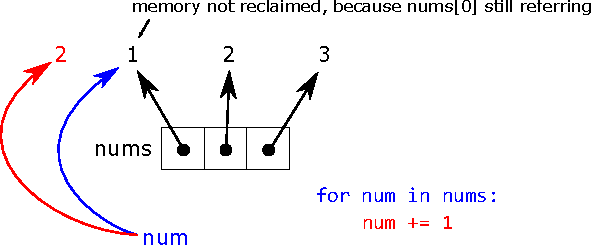
\includegraphics[width=250px]{./img/name_value_1.pdf}
\captionof{figure}{\label{fig:org5dba91c}
Try to change value referenced in list}
\end{center}
\subsubsection{Example 2}
\label{sec:org21099df}
\begin{minted}[linenos,firstnumber=1,breaklines=true,breakanywhere=true]{python}
nums = [[1], [2], [3]]

for num in nums:
    num[0] += 1
    print(num)
print(nums)

\end{minted}
Output:
\begin{verbatim}
[2]
[3]
[4]
[[2], [3], [4]]
\end{verbatim}

The process can be shown below:
\begin{center}
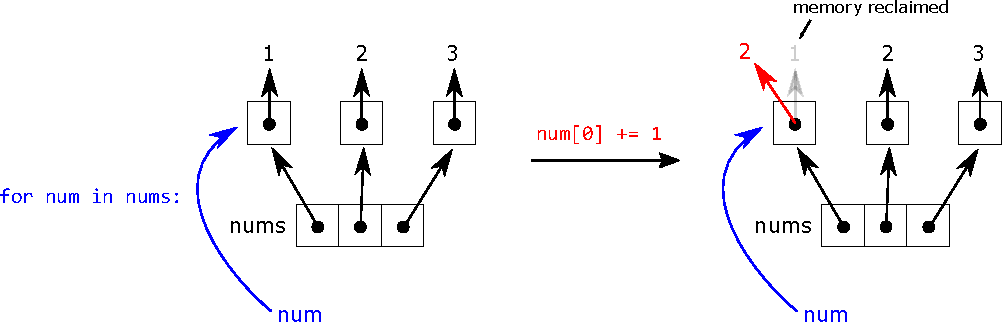
\includegraphics[width=500px]{./img/name_value_2.pdf}
\captionof{figure}{\label{fig:orgbfa4dca}
Try to change value referenced in list of list}
\end{center}

An unreferenced value will be reclaimed by python. To demonstrate this, we can use another variable to reference one of the value originally referenced by the list of list:
\begin{minted}[linenos,firstnumber=1,breaklines=true,breakanywhere=true]{python}
nums = [[1], [2], [3]]
first_num = nums[0][0]  # keep reference

for num in nums:
    num[0] += 1
    print(num)
print(nums)

print(first_num)  # check original value's existence
\end{minted}
Output:
\begin{verbatim}
[2]
[3]
[4]
[[2], [3], [4]]
1
\end{verbatim}

The process is shown below:
\begin{center}
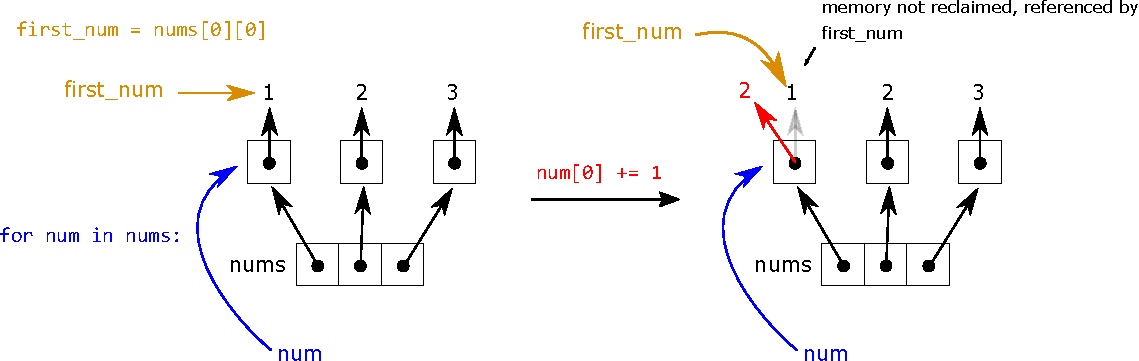
\includegraphics[width=500px]{./img/name_value_3.pdf}
\captionof{figure}{\label{fig:orgfe13190}
Try to keep value from being reclaimed}
\end{center}
\subsection{Type Annotations}
\label{sec:org8e62a6b}
Python is a gradual typing system. It allows not only dynamical typing but also static typing. It uses type annotations (also known as type hints) to allows one to specify types of variables and function arguments/return values. The syntax is as follows:
\begin{minted}[linenos,firstnumber=1,breaklines=true,breakanywhere=true]{python}
my_variable: int # variable annotation

# function annotation
def greeting(name: str) -> str:
    return 'Hello ' + name
\end{minted}
The \texttt{-> str} part has annotated the return type of the function.

However, you can still assign different types to a variable that is annoted otherwise. Python will still run (although in pycharm, IDE will notify you of the unmatched type issue).
\subsection{Pylint}
\label{sec:org7f19224}
Pylint is a python source code analyzer that helps you maintain good coding standards.
\section{Bool Value}
\label{sec:org4527f0f}
In Python, the two bool values are:
\begin{minted}[breaklines=true,breakanywhere=true]{python}
True
False
\end{minted}
Notice that, the first letter is capitalized. Unlike in C++ (\texttt{true, false}).
\section{String}
\label{sec:org9000cb7}
String is a sequence of characters in python. String is immutable. The python string documentation can be found \href{https://docs.python.org/3/library/string.html}{here}.
\subsection{String Formating}
\label{sec:org733d03a}
Placing 'r' before a string will yield its raw value. For example:
\begin{minted}[linenos,firstnumber=1,breaklines=true,breakanywhere=true]{python}
print(r"\n\n\n")
\end{minted}
Output:
\begin{verbatim}
\n\n\n
\end{verbatim}

\subsection{Access Single Character by []}
\label{sec:orgcf738a3}
Just like string in C++, you can access the individual character in a string by using \texttt{[]}. For example:
\begin{minted}[linenos,firstnumber=1,breaklines=true,breakanywhere=true]{python}
content = "abcde"
print(content[0])
\end{minted}
Output:
\begin{verbatim}
a
\end{verbatim}

The indexing of string also supports negative index. Check List section in this notes for more details. For example:
\begin{minted}[breaklines=true,breakanywhere=true]{python}
content = "abcde"
print(content[-1])
print(content[-3])
\end{minted}
Output:
\begin{verbatim}
e
c
\end{verbatim}

One key difference between python string and C++ string is that, you can't modify the single character in string by the bracket operator. For example:
\begin{minted}[linenos,firstnumber=1,breaklines=true,breakanywhere=true]{python}
string = "abcde"
string[0] = 'a'
\end{minted}
Output:
\begin{verbatim}
TypeError: 'str' object does not support item assignment
\end{verbatim}

\subsection{Functions}
\label{sec:orgdafd844}
\subsubsection{General Idea}
\label{sec:org73df152}
Just like string class in C++, a data type in python has member functions. This is even true for primitive types in C++ (for example, \texttt{int, double}), i.e. these "primitive" types also have their own member functions.

To call the member function in python's data type, you use \texttt{.} operator (same as C++):
\begin{minted}[linenos,firstnumber=1,breaklines=true,breakanywhere=true]{python}
content = "abc"
print(content.isupper())
\end{minted}
In the above code, the function \texttt{isupper()} will return a Boolean value indicating whether the string variable contains all upper case letters. In this case, the result would be:
\begin{verbatim}
False
\end{verbatim}

You can concatenate the calling of member functions. For example:
\begin{minted}[linenos,firstnumber=1,breaklines=true,breakanywhere=true]{python}
content = "abc123"
print(content.upper().isupper())
print(content)
\end{minted}
In line 2, the member function \texttt{upper()} of the string variable \texttt{content} is called first. This function will return a string variable which contains the copy of \texttt{content} variable, except that all lower case letters are transformed to upper case letters. Then, the member function \texttt{isupper()} of this \textbf{RETURNED} variable will be called to check if all letters in this \textbf{RETURNED} variable are upper case. After this, in line 3, \texttt{content} will be printed again to show the data stored in \texttt{content} hasn't been changed by the \texttt{upper()} member function. The output is:
\begin{verbatim}
True
abc123
\end{verbatim}

Some often used member functions and global functions are listed in the following sections.
\subsubsection{\texttt{float()}}
\label{sec:org4bd8c7d}
This global function will convert a string into a float number, and will return this number. The input string must be only in the format of a float number, i.e. either x or x.x, where x can be only digit, otherwise, errors will be thrown.

Example:
\begin{minted}[linenos,firstnumber=1,breaklines=true,breakanywhere=true]{python}
num = input("Enter a number: ")
print(float(num))
\end{minted}
Output:
\begin{verbatim}
Enter a number; 5.5
5.5
\end{verbatim}
\subsubsection{\texttt{int()}}
\label{sec:org86f609f}
This global function will convert a string into an integer number, and will return this number. The input string must contain only digit, otherwise, errors will be thrown.

Example:
\begin{minted}[linenos,firstnumber=1,breaklines=true,breakanywhere=true]{python}
num = input("Enter a number: ")
print(int(num))
\end{minted}
Output:
\begin{verbatim}
Enter a number; 5
5
\end{verbatim}
\subsubsection{\texttt{len()}}
\label{sec:orgd4778cd}
This function will return an integer that indicates the length of a string variable \texttt{string}. It is \textbf{not} a member function of string, but a global function, which accepts "sized" parameter in python (iterable object).
\subsubsection{\texttt{.count()}}
\label{sec:org3ac6019}
This function accepts a string, it will return an integer that indicates the number of times the string appeared in the calling string. Example:
\begin{minted}[linenos,firstnumber=1,breaklines=true,breakanywhere=true]{python}
string = "abcdede"
print("Counting result : ", string.count("de"))
\end{minted}
Output:
\begin{verbatim}
Counting result :  2
\end{verbatim}
\subsubsection{\texttt{.index()}}
\label{sec:org357f8c5}
This member function will return the starting index value of a character or sub-string in the string (first appearing position). For example:
\begin{minted}[linenos,firstnumber=1,breaklines=true,breakanywhere=true]{python}
string = "abcd 123 apple"
print(string.index(" "))
print(string.index(" ap"))
\end{minted}
Output:
\begin{verbatim}
4
8
\end{verbatim}

When the parameter (character or substring) is not in the string, an error will be thrown:
\begin{minted}[linenos,firstnumber=1,breaklines=true,breakanywhere=true]{python}
string = "abcd 123 apple"
print(string.index("pee"))
\end{minted}
Output:
\begin{verbatim}
ValueError: substring not found
\end{verbatim}
The code lines that are after this line will not be executed, program will stop.
\subsubsection{\texttt{.islower()}}
\label{sec:org5669a37}
This function will return a Boolean value to check if \textbf{ALL} letters in \texttt{string} are lowercase. Its a member function of string.
\subsubsection{\texttt{.isupper()}}
\label{sec:org0ad0dd5}
This function will return a Boolean value to check if \textbf{ALL} letters in \texttt{string} are uppercase. Its a member function of string.
\subsubsection{\texttt{.join()}}
\label{sec:org6c85917}
This function accepts an iterable sequence object. It will return a string which is built using following logic: concatenate iterated item in the sequence and the original string to make a combined string, this is done for each of the item in the sequence. Then return the combination of all these strings. For example, if the sequence is \texttt{['1', '2', '3']}, and the calling string is: \texttt{"abc"}, then following substrings will be first made;
\begin{itemize}
\item \texttt{"1abc"}
\item \texttt{"2abc"}
\item \texttt{"3abc"}
\end{itemize}
Then they will be combined to gether to give: \texttt{"1abc2abc3abc"}.

Example:
\begin{minted}[linenos,firstnumber=1,breaklines=true,breakanywhere=true]{python}
t1 = ('c', 't', 'y')
string = "123"
print(string.join(t1))
\end{minted}
Output:
\begin{verbatim}
c123t123y
\end{verbatim}

This function can be used to convert a list to a string, just choose an empty string to call the \texttt{.join()} function:
\begin{minted}[linenos,firstnumber=1,breaklines=true,breakanywhere=true]{python}
t1 = ('c', 't', 'y')
print("".join(t1))
\end{minted}

\subsubsection{\texttt{.lower()}}
\label{sec:org3605329}
This function will return a copy of \texttt{string} with all letters lower cased. It is useful for storing data: transform your string data into lower case so you can manage them with ease.
\subsubsection{\texttt{.replace()}}
\label{sec:org2e20e2e}
This function accepts two string parameters:
\begin{minted}[breaklines=true,breakanywhere=true]{python}
string.replace("search_key", "replace_key")
\end{minted}

It will search for the existence of \texttt{"search\_key"} in the string. If the key being found, it will be replaced by \texttt{"replace\_key"}. This "replaced" version of the string will be returned by this function (as a copy of the original string). For example:
\begin{minted}[linenos,firstnumber=1,breaklines=true,breakanywhere=true]{python}
content = "accab"
print(content.replace("a", "c"))
print(content)
\end{minted}
Output:
\begin{verbatim}
ccccb
accab
\end{verbatim}
When no match found, no error will be thrown. Code lines followed will be executed.
\subsubsection{\texttt{.title()}}
\label{sec:org8cef1c7}
Change the first letter of each word into upper case. Example:
\begin{minted}[linenos,firstnumber=1,breaklines=true,breakanywhere=true]{python}
string = "this is a title"
print(string.title())
\end{minted}
Output:
\begin{verbatim}
This Is A Title
\end{verbatim}

\subsubsection{\texttt{.rstrip()} and \texttt{.lstrip()}}
\label{sec:orgfa09f4c}
This function will return a string that stripped any whitespaces on the right or left side of the \texttt{self} string. For example:
\begin{minted}[linenos,firstnumber=1,breaklines=true,breakanywhere=true]{python}
string = ["\tthis is a title    "]
print("Before: ", string)
print("After .rstrip(): ", [string[0].rstrip()])
print("After .lstrip(): ", [string[0].lstrip()])
\end{minted}
Output:
\begin{verbatim}
Before:  ['\tthis is a title    ']
After .rstrip():  ['\tthis is a title']
After .lstrip():  ['this is a title    ']
After both:  ['this is a title']
\end{verbatim}

To strip the whitespaces at right end and left end simultaneously, you can use \texttt{.strip()}. In the real world, these stripping functions are used most often to clean up user input before it’s stored in a program.
\subsubsection{\texttt{.split()}}
\label{sec:orge977883}
This method separates the string into substrings wherever it finds a space and stores all the substrings in a list. For example:
\begin{minted}[linenos,firstnumber=1,breaklines=true,breakanywhere=true]{python}
title = "Alice in Wonderland!"
print(title.split())
\end{minted}
Output:
\begin{verbatim}
['Alice', 'in', 'Wonderland!']
\end{verbatim}

\subsubsection{\texttt{.upper()}}
\label{sec:orgc2e6b68}
This function will return a copy of \texttt{string} with all letters upperized. Its a member function of string.

\subsubsection{\texttt{in, not in}}
\label{sec:org8e39268}
Check if a character is in a string. Example:
\begin{minted}[linenos,firstnumber=1,breaklines=true,breakanywhere=true]{python}
str1 = "abc"
str2 = "1234"
print('1' in str2)
print('d' in str1)
\end{minted}
Output:
\begin{verbatim}
True
False
\end{verbatim}

\subsection{Chinese Support in Python String}
\label{sec:orgc2136bf}
Unlike C++'s string class which needs to specify different encoding system in order to hold Chinese characters, you can directly assign Chinese character to a python variable.
\subsection{Operators}
\label{sec:org4cc9b2c}
\subsubsection{\texttt{*}}
\label{sec:org2dbff57}
String only accepts multiply by an integer. \texttt{str * i} will return a new string, which is \texttt{str} repeated \texttt{i} times. For example:
\begin{minted}[linenos,firstnumber=1,breaklines=true,breakanywhere=true]{python}
print("abcde0" * 3)
\end{minted}
Output:
\begin{verbatim}
abcde0abcde0abcde0
\end{verbatim}
\subsubsection{\texttt{+}}
\label{sec:orga7b3c8a}
Concatenate the string with another string. For example:
\begin{minted}[linenos,firstnumber=1,breaklines=true,breakanywhere=true]{python}
print("abcde0" + '2')
\end{minted}
Output:
\begin{verbatim}
abcde02
\end{verbatim}

\section{Numerics}
\label{sec:org6c055e5}
The subtypes are int, float and complex.
\subsection{Functions}
\label{sec:org3737a36}
\subsubsection{\texttt{str(num)}}
\label{sec:orgf76f7d4}
You can use this global function to convert a number variable to a string object. It will return the string version of the number variable. For example:
\begin{minted}[linenos,firstnumber=1,breaklines=true,breakanywhere=true]{python}
num = 5.45
print(str(num).index("."))
\end{minted}

Output:
\begin{verbatim}
1
\end{verbatim}
\subsubsection{\texttt{abs(num)}}
\label{sec:orgd681cb7}
This global function will return a copy of the abusolute value of \texttt{num}. Also, there is a member function can do the same thing:
\begin{minted}[linenos,firstnumber=1,breaklines=true,breakanywhere=true]{python}
num = -5.35
print(abs(num))
print(num.__abs__())
\end{minted}
Output:
\begin{verbatim}
5.35
5.35
\end{verbatim}

\subsubsection{\texttt{pow()}}
\label{sec:org4e66802}
A global function that accepts two parameters: \texttt{pow(base, exponent)}. It will return the result.
\begin{minted}[linenos,firstnumber=1,breaklines=true,breakanywhere=true]{python}
print(pow(2, 3))
\end{minted}
Output:
\begin{verbatim}
8
\end{verbatim}

\subsubsection{\texttt{max()}}
\label{sec:orgcfc3743}
This global function will return a copy of the maximum numbers in the passed in parameter. For example:
\begin{minted}[linenos,firstnumber=1,breaklines=true,breakanywhere=true]{python}
print(max(2, -1, 3, 5, 6, 1, 2, 10))
\end{minted}
Output:
\begin{verbatim}
10
\end{verbatim}

\subsubsection{\texttt{min()}}
\label{sec:org461d740}
This global function will return a copy of the minimum numbers in the passed in parameter. For example:
\begin{minted}[linenos,firstnumber=1,breaklines=true,breakanywhere=true]{python}
print(min(2, -1, 3, 5, 6, 1, 2, 10))
\end{minted}
Output:
\begin{verbatim}
10
\end{verbatim}

\subsubsection{\texttt{round()}}
\label{sec:org77c79a3}
This global function will return a copy of the closest integer of the number passed in. For example:
\begin{minted}[breaklines=true,breakanywhere=true]{python}
print(round(2.36))
print(round(-2.45))
print(round(-3.1))
\end{minted}
Output:
\begin{verbatim}
2
-2
-3
\end{verbatim}

\subsubsection{\texttt{math::floor()}}
\label{sec:org474d3e7}
This function is defined in \texttt{math} module. It will return the integer that is no larger than the input parameter. For example:
\begin{minted}[linenos,firstnumber=1,breaklines=true,breakanywhere=true]{python}
from math import *
print(floor(2.4))
\end{minted}
Output:
\begin{verbatim}
2
\end{verbatim}

\subsubsection{\texttt{math::ceil()}}
\label{sec:orgb4330aa}
This function is defined in \texttt{math} module. It will return the integer that is no smaller than the input parameter. For example:
\begin{minted}[linenos,firstnumber=1,breaklines=true,breakanywhere=true]{python}
from math import *
print(ceil(2.4))
\end{minted}
Output:
\begin{verbatim}
3
\end{verbatim}

\subsubsection{\texttt{math::sqrt()}}
\label{sec:orgafdfb79}
This function is defined in \texttt{math} module. It will return the square root of the input parameter. For example:
\begin{minted}[linenos,firstnumber=1,breaklines=true,breakanywhere=true]{python}
from math import *
print(sqrt(4))
\end{minted}
Output:
\begin{verbatim}
2
\end{verbatim}

\chapter{Data Structures}
\label{sec:org545509c}
\section{Sequence}
\label{sec:orgd40c18e}
\subsection{General Idea}
\label{sec:org853160d}
Sequence is not a specific type of data structure. It is the iterable type, which means it is composed of smaller pieces of information, and these information are stored inside a single entity (sequence).

There are seven sequence subtypes:
\begin{itemize}
\item strings
\item lists
\item tuples
\item sets
\item bytes
\item bytearrays
\item range objects
\end{itemize}

The range data type finds common use in the construction of enumeration-controlled loops.
\subsection{Common Sequence Operations (for both immutable and mutable)}
\label{sec:org01cf695}
\subsubsection{\texttt{x in s}}
\label{sec:org7e94090}
\texttt{True} if an item of is is equal to \texttt{x}, else \texttt{False}
\subsubsection{\texttt{x not in s}}
\label{sec:org8d5b994}
\texttt{False} if an item of \texttt{s} is equal to \texttt{x}, else \texttt{True}
\subsubsection{\texttt{s + t}}
\label{sec:org7943d8b}
The concatenation of \texttt{s} and \texttt{t}
\subsubsection{\texttt{s * n}, \texttt{n * s}}
\label{sec:orga815722}
\texttt{n} shallow copies of \texttt{s} concatenated
\subsubsection{\texttt{s[i]}}
\label{sec:org8bfc500}
\texttt{i} th items of \texttt{s}, start from 0
\subsubsection{\texttt{s[i:j]}}
\label{sec:orged5aa98}
Slice of \texttt{s} from \texttt{i} to \texttt{j}
\subsubsection{\texttt{s[i:j:k]}}
\label{sec:orgef64f3c}
Slice of \texttt{s} from \texttt{i} to \texttt{j} with step \texttt{k}
\subsubsection{\texttt{len(s)}}
\label{sec:org2a0e3e2}
Length of \texttt{s}
\subsubsection{\texttt{min(s)}}
\label{sec:orgcbe1683}
Smallest item of \texttt{s}
\subsubsection{\texttt{max(s)}}
\label{sec:org513d481}
Largest item of \texttt{s}
\subsubsection{\texttt{s.index(x)}}
\label{sec:orgcc55aae}
Index of the first occurrence of \texttt{x} in \texttt{s}. If \texttt{x} not found in \texttt{s}, a \texttt{ValueError} will be thrown (\texttt{ValueError: substring not found}).
\subsubsection{\texttt{s.count(x)}}
\label{sec:org8c91085}
Total number of occurrences of \texttt{x} in \texttt{s}. If \texttt{x} not found in \texttt{s}, no error thrown, just return 0.
\subsection{Mutable Sequence Operations}
\label{sec:orgf1858ae}
\subsubsection{\texttt{s[i] = x}}
\label{sec:orge623127}
Item \texttt{s[i]} of \texttt{s} is replaced by \texttt{x}. Here, \texttt{x} will be evaluated as an object. If \texttt{x} is a sequence, it will replace \texttt{s[i]} as a whole. For example:
\begin{minted}[linenos,firstnumber=1,breaklines=true,breakanywhere=true]{python}
list1 = [x for x in range(3, 15, 2)]
list2 = [2, 4, 6, 8, 10]

print(list1)
list1[1] = list2
print(list1)
\end{minted}
Output:
\begin{verbatim}
[3, 5, 7, 9, 11, 13]
[3, [2, 4, 6, 8, 10], 7, 9, 11, 13]
\end{verbatim}
\subsubsection{\texttt{s[i:j] = []}}
\label{sec:orge763890}
Delete slice of \texttt{s} from \texttt{i} to \texttt{j} (not including \texttt{s[j]}). For example:
\begin{minted}[linenos,firstnumber=1,breaklines=true,breakanywhere=true]{python}
list1 = [x for x in range(3, 15, 2)]
print(list1)
list1[:4] = []
print(list1)
\end{minted}
Output:
\begin{verbatim}
[3, 5, 7, 9, 11, 13]
[11, 13]
\end{verbatim}
\subsubsection{\texttt{s[i:j] = t}}
\label{sec:org283f822}
Slice of \texttt{s} from \texttt{i} to \texttt{j} (not including \texttt{s[j]}) is replaced by the contents of \texttt{t}, \texttt{len(s[i:j])} and \texttt{len(t)} does not need to be equal. Here, \texttt{t} will be evaluated as a sequence. This statement will produce same result as if you go following steps:
\begin{itemize}
\item call \texttt{s[i:j] = []} to delete slice of \texttt{s} from \texttt{i} to \texttt{j}
\item for each iterated item in \texttt{t}, insert them starting from \texttt{i}
\end{itemize}

Example:
\begin{minted}[linenos,firstnumber=1,breaklines=true,breakanywhere=true]{python}
list1 = [x for x in range(3, 15, 2)]
dic1 = {
    'a': "A",
    'b': "B",
    'c': "C"
}

print(list1)
list1[:4] = dic1
print(list1)
\end{minted}
Output:
\begin{verbatim}
[3, 5, 7, 9, 11, 13]
['a', 'b', 'c', 11, 13]
\end{verbatim}
Pay attention that, in a set of key-value pair (i.e. dictionary), only key will be inserted. Also notice that, Slice \texttt{list1[:4]} has been deleted, and only three entries added, the size of \texttt{list1} is reduced by 1.

Another example showing that \texttt{t} is evaluated as an iterable sequence rather than a whole object:
\begin{minted}[linenos,firstnumber=1,breaklines=true,breakanywhere=true]{python}
list1 = [x for x in range(3, 15, 2)]
str1 = 'abcdef'

print(list1)
list1[:4] = str1
print(list1)
\end{minted}
Output:
\begin{verbatim}
[3, 5, 7, 9, 11, 13]
['a', 'b', 'c', 'd', 'e', 'f', 11, 13]
\end{verbatim}
So \texttt{str1} is inserted one character at a time (each iterated item is a character).

\subsubsection{\texttt{s[i:j:k] = t}}
\label{sec:org09eb700}
The elements of \texttt{s[i:j:k] are replaced by those of \textasciitilde{}t}. Pay attention that the number of elements in slice \texttt{s[i:j:k]} should be equal to number of elements in \texttt{t}. Otherwise, \texttt{ValueError} will be thrown (attempt to assign sequence of size \texttt{len(t)} to extended slice of size \texttt{len(s[i:j:k])}).

Example:
\begin{minted}[linenos,firstnumber=1,breaklines=true,breakanywhere=true]{python}
list1 = [x for x in range(3, 18, 2)]
print(list1)
list1[:5:2] = [0, 0, 0]
print(list1)
\end{minted}
Output:
\begin{verbatim}
[3, 5, 7, 9, 11, 13, 15, 17]
[0, 5, 0, 9, 0, 13, 15, 17]
\end{verbatim}

\subsubsection{\texttt{del s[i:j]} and \texttt{del s[i:j:k]}}
\label{sec:org72fd150}
Delete the slice in \texttt{s} indicated by \texttt{[i:j]} and \texttt{[i:j:k]}.
\subsubsection{\texttt{s.append(x)}}
\label{sec:org98f52b6}
Add \texttt{x} to the end of \texttt{s}, here \texttt{x} will be evaluated as an object, not a sequence. It will be appended to \texttt{s} as a whole. Example:
\begin{minted}[linenos,firstnumber=1,breaklines=true,breakanywhere=true]{python}
list1 = [2, 4, 6, 8, 10]
str1 = 'abcdef'
print(list1)
list1.append(str1)
print(list1)
\end{minted}
Output:
\begin{verbatim}
[2, 4, 6, 8, 10]
[2, 4, 6, 8, 10, 'abcdef']
\end{verbatim}
\subsubsection{\texttt{s.clear()}}
\label{sec:org607c28d}
This will clear the content stored in a sequence.
\subsubsection{\texttt{s.count(x)}}
\label{sec:org463a1b4}
Return number of occurrence of \texttt{x} in \texttt{s}.

\subsubsection{\texttt{s.extend(x)}}
\label{sec:org0381b63}
Append the content of \texttt{x} to end of \texttt{s}. Here, \texttt{x} will be evaluated as a iterable sequence. It is doing the same thing as:
\begin{minted}[linenos,firstnumber=1,breaklines=true,breakanywhere=true]{python}
for item in x:
    s.append(item)
\end{minted}
Example:
\begin{minted}[linenos,firstnumber=1,breaklines=true,breakanywhere=true]{python}
list1 = [2, 4, 6, 8, 10]
str1 = 'abcdef'
print(list1)
list1.extend(str1)
print(list1)
\end{minted}
Output:
\begin{verbatim}
[2, 4, 6, 8, 10]
[2, 4, 6, 8, 10, 'a', 'b', 'c', 'd', 'e', 'f']
\end{verbatim}

\subsubsection{\texttt{s.insert(i, x)}}
\label{sec:org2fe9991}
Insert \texttt{x} at position \texttt{i}.

\subsubsection{\texttt{s.pop()}}
\label{sec:orgb33e489}
This function will remove the last item in the sequence (default operation, when no parameters passed in). Example:
\begin{minted}[linenos,firstnumber=1,breaklines=true,breakanywhere=true]{python}
name = ["what", "a", "big", "apple"]
print("Before pop: ", name)
name.pop()
print("After pop: ", name)
\end{minted}
Output:
\begin{verbatim}
Before clear:  ['what', 'a', 'big', 'apple']
After clear:  ['what', 'a', 'big']
\end{verbatim}

This function will return the popped item, you can declare a variable to hold it and do more stuff with it:
\begin{minted}[linenos,firstnumber=1,breaklines=true,breakanywhere=true]{python}
popped_item = items.pop()
\end{minted}

When an integer value \texttt{i} is passed in, the item at that index will be popped (and returned):
\begin{minted}[linenos,firstnumber=1,breaklines=true,breakanywhere=true]{python}
items.pop(1)
\end{minted}
The second item in the list will be popped.
\subsubsection{\texttt{s.remove()}}
\label{sec:orgea46e79}
Same as \texttt{del s[s.index(x)]}. If \texttt{x} is not in the list, \texttt{ValueError} will be thrown.
\subsubsection{\texttt{s.reverse()}}
\label{sec:orgcbc762b}
Reverses the items of \texttt{s} in place
\subsubsection{\texttt{s.sort()}}
\label{sec:org0f2a85a}
This function will sort the sequence in ascending order. For example:
\begin{minted}[linenos,firstnumber=1,breaklines=true,breakanywhere=true]{python}
nums = [3, 2, 7, 1, 5]
nums.sort()
print(nums)
\end{minted}
Output:
\begin{verbatim}
[1, 2, 3, 5, 7]
\end{verbatim}

It will use a compare function to determine the order of the item. The comparator should define ordering information among any two pairs of the elements stored in the list. If not, an error will be thrown. For example:
\begin{minted}[linenos,firstnumber=1,breaklines=true,breakanywhere=true]{python}
name = ["what", "a", "big", "Apple", 2]
name.sort()
print(name)
\end{minted}
Output:
\begin{verbatim}
TypeError: '<' not supported between instances of 'int' and 'str'
\end{verbatim}

To sort the items reversely (in descending order), you pass \texttt{reverse = True} into the \texttt{sort()} function. For example:
\begin{minted}[linenos,firstnumber=1,breaklines=true,breakanywhere=true]{python}
nums = [1, 2, 3, 4, 5]
nums.sort(reverse=True)
print(nums)
\end{minted}
Output:
\begin{verbatim}
[5, 4, 3, 2, 1]
\end{verbatim}
\section{Iterators and Iterables \label{org49c6fd0}}
\label{sec:org7ac6502}
\href{https://www.geeksforgeeks.org/python-difference-iterable-iterator/}{Reference}

Iterator is an object, which is used to iterate over an iterable object using \texttt{\_\_next\_\_()} method. This method returns the next item of the object. 

Iterable is an object, which can be iterated over. If you pass an iterable to \texttt{iter()} method, an iterator of this iterable object will be returned.

An iterator type should have following methods defined:
\begin{itemize}
\item \texttt{\_\_next\_\_()}: return next item in the iterator
\item \texttt{\_\_iter\_\_()}: this is called when initializing an iterator using an iterable. This should return an object that has a \texttt{\_\_next\_\_()} method (an iterator). This function will be tried to be called by python when an object is passed into global \texttt{iter()} function.
\end{itemize}

Note that, every iterator is also an iterable (if you call \texttt{iter()} and pass in an iterator, it will return itself, same memory address, as if you defined an alias for the passed-in iterator). However, not every iterable is an iterator (because some iterables may not have \texttt{\_\_next\_\_()} and \texttt{\_\_iter\_\_()} defined).

An example of using iterator can be found in \hyperref[org900c2e7]{details of for loop}.
\section{List}
\label{sec:org78c3e5b}
List is a way of managing data in python. Because a list usually contains more than one element, it’s a good idea to make the name of your list plural, such as letters, digits, or names.
\subsection{Declaration}
\label{sec:org316c950}
\subsubsection{Declare by Constructed List}
\label{sec:orgba22a4b}
To declare a list:
\begin{minted}[linenos,firstnumber=1,breaklines=true,breakanywhere=true]{python}
friend = ["A", "B", "C"]
\end{minted}
The \texttt{[]} will indicate a list structure. So basically the computer knows that a bunch of values will be stored in \texttt{friend}.

Unlike arrays in C++, you can put different types into a same list, for example:
\begin{minted}[linenos,firstnumber=1,breaklines=true,breakanywhere=true]{python}
friend = ["A", "B", 2, 2.5, "C"]
print(friend[1])
print(friend[-2])
\end{minted}
Output:
\begin{verbatim}
B
2.5
\end{verbatim}

You can print the whole list by passing the name of the list into \texttt{print()}, for example:
\begin{minted}[linenos,firstnumber=1,breaklines=true,breakanywhere=true]{python}
friend = ["A", "B", 2, 2.5, "C"]
print(friend)
\end{minted}
Output:
\begin{verbatim}
['A', 'B', 2, 2.5, 'C']
\end{verbatim}
Notice that for non-string element, there is no \texttt{'} (which indicates string object).
\subsubsection{Declare by another List}
\label{sec:org333a948}
Suppose you have two lists \texttt{A} and \texttt{B}, and \texttt{B} is declared using \texttt{=} directly:
\begin{minted}[linenos,firstnumber=1,breaklines=true,breakanywhere=true]{python}
A = [1, 2, 3, 4, 5]
B = A
\end{minted}
In python, line 2 is actually defining a left-reference of \texttt{A}, named \texttt{B}. They are referencing to the same memory space that hold \texttt{[1, 2, 3, 4, 5]}. So, for example, if \texttt{A} is reversed, then print \texttt{B}, it is also reversed:
\begin{minted}[linenos,firstnumber=1,breaklines=true,breakanywhere=true]{python}
A.reverse()
print(B)
\end{minted}
Output:
\begin{verbatim}
[5, 1, 7, 2, 3]
\end{verbatim}

To copy the content in \texttt{A} to \texttt{B}, you need to use the \texttt{.copy()} member function:
\begin{minted}[linenos,firstnumber=1,breaklines=true,breakanywhere=true]{python}
B = A.copy()
\end{minted}

You can also call the built-in list constructor and pass in the list you want to duplicate. A copy of the argument list will be created and returned:
\begin{minted}[linenos,firstnumber=1,breaklines=true,breakanywhere=true]{python}
B = list(A)
\end{minted}

\subsection{\texttt{operator[]}}
\label{sec:orgeed7aa4}
The specific element can be accessed by the \texttt{[]} operator. The indexing is similar with C++, from \texttt{0} to \texttt{size - 1}. However, python also supports indexing from \texttt{-1} to \texttt{-size}, the position these negative indexes \texttt{i} refered to is the same as \texttt{size + i}, so \texttt{-1} is the last element, while \texttt{-size} is the first element. 


You can select portion of the list by using \texttt{:}. When you type \texttt{array[a:b]}, it will return a subarray, which is portion of the original \texttt{array}, where the subarray contains elements in range \texttt{[a,b)}, notice: not including the ending element. For example:
\begin{minted}[linenos,firstnumber=1,breaklines=true,breakanywhere=true]{python}
nums = [1, 2, 3, 4, 5, "end"]
print(nums[2:4])
\end{minted}
Output:
[3, 4]
\subsection{\texttt{in} keyword}
\label{sec:orgedb6fa1}
You can use \texttt{in} to determine whether an element is inside the list or not. For example:
\begin{minted}[linenos,firstnumber=1,breaklines=true,breakanywhere=true]{python}
nums = [1, 1, 2, 2, 1, 3, 4, 6, 7, 9]
print(1 in nums)
\end{minted}
Output:
\begin{verbatim}
True
\end{verbatim}

This expression can be used in many situations, like \texttt{if} statement, \texttt{while} loop (looping condition).

\subsection{Slice}
\label{sec:orge7b04c6}
You can use slice to get a copy of portions of the list by using colon. For example: \texttt{array[a:]}, this will return a sublist that begin at \texttt{a}, all the way to the last element of the array. For example:
\begin{minted}[linenos,firstnumber=1,breaklines=true,breakanywhere=true]{python}
nums = [1, 2, 3, 4, 5, "end"]
print(nums[2:])
\end{minted}
Output:
\begin{verbatim}
[3, 4, 5, 'end']
\end{verbatim}

If you omit the first index in a slice, python automatically starts your slice at the beginning of the list. For example:
\begin{minted}[linenos,firstnumber=1,breaklines=true,breakanywhere=true]{python}
nums = [i for i in range(1, 10)]
print(nums[:5])
\end{minted}
Output:
\begin{verbatim}
[1, 2, 3, 4, 5]
\end{verbatim}

Slice also works for negative index. If left of the slice is omitted, it means from start to where the negative index refer to. If right of the slice is omitted, it means from where the negative index refer to, to the end. Example:
\begin{minted}[linenos,firstnumber=1,breaklines=true,breakanywhere=true]{python}
nums = [i for i in range(1, 10)]
print(nums[:-3])
print(nums[-3:])
\end{minted}
Output:
\begin{verbatim}
[1, 2, 3, 4, 5, 6]
[7, 8, 9]
\end{verbatim}

Slice can be used in for loop (as the iterated object). For example, to loop through the first three element in a list:
\begin{minted}[linenos,firstnumber=1,breaklines=true,breakanywhere=true]{python}
nums = [i for i in range(1, 10)]
for num in nums[:3]:
    print(num)
\end{minted}
Output:
\begin{verbatim}
1
2
3
\end{verbatim}

\subsection{List comprehension \label{org3b2d900}}
\label{sec:orgc75dd05}
A list comprehension combines the \texttt{for} loop and the creation of new elements into one line, so you can make a list in a simple way. The syntax is as follows:
\begin{minted}[linenos,firstnumber=1,breaklines=true,breakanywhere=true]{python}
nums = [i*i for i in range(1, 10)]
\end{minted}
Output:
\begin{verbatim}
[1, 4, 9, 16, 25, 36, 49, 64, 81]
\end{verbatim}

The general form of a list comprehension is like:
\begin{minted}[linenos,firstnumber=1,breaklines=true,breakanywhere=true]{python}
[expression for x in sequence]
\end{minted}
You can put any sequence in \texttt{sequence}, such as a function call that will return a sequence.

Below are more complicated examples to use list comprehensions:
\begin{minted}[linenos,firstnumber=1,breaklines=true,breakanywhere=true]{python}
squares = [(x, x**2, x**3) for x in range(0,9) if x % 2 == 0]
print(squares)
\end{minted}
Output:
\begin{verbatim}
[(0, 0, 0), (2, 4, 8), (4, 16, 64), (6, 36, 216), (8, 64, 512)]
\end{verbatim}

You can even use nested list comprehension:
\begin{minted}[linenos,firstnumber=1,breaklines=true,breakanywhere=true]{python}
list_num = [[x*y for x in range(1,5)] for y in range(1,5)]
print(list_num)
\end{minted}
Output:
\begin{verbatim}
[[1, 2, 3, 4], [2, 4, 6, 8], [3, 6, 9, 12], [4, 8, 12, 16]]
\end{verbatim}

\subsection{2D List}
\label{sec:org23828b8}
The idea of 2D list is simple. It is a list, whose element object is another list. For example:
\begin{minted}[linenos,firstnumber=1,breaklines=true,breakanywhere=true]{python}
matrix = [
    [1, 2, 3],
    [4, 5, 6],
    [7, 8, 9],
    [0]
]
\end{minted}

Each list object is a row in the 2D matrix. Each object in each row list is the column of the 2D matrix. To access the specific element, we use double bracket operator. For example, assume the above matrix is declared, then \texttt{matrix[0][2] == 3}.

Example: use a nested for loop to traverse the 2D lists defined above. We have two ways, the first one is to use bracket operator:
\begin{minted}[linenos,firstnumber=1,breaklines=true,breakanywhere=true]{python}
for row in range(len(matrix)):
    for column in range(len(matrix[row])):
	print(matrix[row][column])
\end{minted}
Output:
\begin{verbatim}
1
2
3
4
5
6
7
8
9
0
\end{verbatim}

The second way is to use range based idea:
\begin{minted}[linenos,firstnumber=1,breaklines=true,breakanywhere=true]{python}
for row in matrix:
    for col in row:
	print(col)
\end{minted}
Output:
\begin{verbatim}
1
2
3
4
5
6
7
8
9
0
\end{verbatim}

\subsection{Functions}
\label{sec:org204026c}
\subsubsection{\texttt{.append()}}
\label{sec:org7f465e5}
Unlike \texttt{.extend()}, you can use \texttt{.append()} to append an object to the calling list. Whatever you put in \texttt{.append()}, it will be interpreted as an object, not an \texttt{iterable}. For example:
\begin{minted}[linenos,firstnumber=1,breaklines=true,breakanywhere=true]{python}
string = "abcde"
nums = [1, 2, 3, 4, 5]
name = ["what", "a", "big", "apple"]
nums.append(string)
nums.append(name[2])
print(nums)
\end{minted}
Output:
\begin{verbatim}
[1, 2, 3, 4, 5, 'abcde', 'big']
\end{verbatim}

If you pass name of another list into it, you will have nested list structure, i.e. one element of the list is another list. For example:
\begin{minted}[linenos,firstnumber=1,breaklines=true,breakanywhere=true]{python}
string = "abcde"
nums = [1, 2, 3, 4, 5]
name = ["what", "a", "big", "apple"]
nums.append(string)
nums.append(name)
print(nums)
\end{minted}
Output:
\begin{verbatim}
[1, 2, 3, 4, 5, 'abcde', ['what', 'a', 'big', 'apple']]
\end{verbatim}
\subsubsection{\texttt{.clear()}}
\label{sec:org32064cc}
This function will clear the content of the list. Example:
\begin{minted}[linenos,firstnumber=1,breaklines=true,breakanywhere=true]{python}
name = ["what", "a", "big", "apple"]
print("Before clear: ", name)
name.clear()
print("After clear: ", name)
\end{minted}
Output:
\begin{verbatim}
Before clear:  ['what', 'a', 'big', 'apple']
After clear:  []
\end{verbatim}
\subsubsection{\texttt{.copy()}}
\label{sec:org990edb1}
This function will return a list, which is the copy of the calling list. Example:
\begin{minted}[linenos,firstnumber=1,breaklines=true,breakanywhere=true]{python}
nums = [3, 2, 7, 1, 5]
nums2 = nums.copy()
nums.reverse()
print(nums2)
\end{minted}
Output:
\begin{verbatim}
[3, 2, 7, 1, 5]
\end{verbatim}

\textbf{More aboud Copying}

Pay attention to how variable works in python. You can't use \texttt{nums2 = nums} to copy \texttt{nums} to \texttt{nums2}, since \texttt{nums2} will reference to the same memory space that actually store the content of the list (which is also referenced by \texttt{nums}).

Another way of copying a list is to use slice:
\begin{minted}[linenos,firstnumber=1,breaklines=true,breakanywhere=true]{python}
nums = [i for i in range(1, 10)]
nums2 = nums[:]
nums.reverse()
print(nums2)
\end{minted}
Output:
\begin{verbatim}
[1, 2, 3, 4, 5, 6, 7, 8, 9]
\end{verbatim}
By not providing begin and end index, the slice will cover the whole list, it will return a \textbf{COPY} of the list (another chunk of memory will hold the copied content). Example:
\begin{minted}[linenos,firstnumber=1,breaklines=true,breakanywhere=true]{python}
nums = [i for i in range(1, 10)]
nums2 = nums[:]
nums.reverse()
print(nums2)
\end{minted}
Output:
\begin{verbatim}
[1, 2, 3, 4, 5, 6, 7, 8, 9]
\end{verbatim}
\subsubsection{\texttt{.count()}}
\label{sec:org2b422e3}
This function accepts an object. It will return an integer showning the number of appearing times in the calling list. Example:
\begin{minted}[linenos,firstnumber=1,breaklines=true,breakanywhere=true]{python}
name = ["what", "a", "big", "apple", 2]
print("Counting result : ", name.count(2))
\end{minted}
Output:
\begin{verbatim}
Counting result :  1
\end{verbatim}

The object type allowed by this function is determined by the type of object the list currently have.
\subsubsection{\texttt{del}}
\label{sec:org0dcbb9e}
\texttt{del} is not a function, but it is a statement that can remove element in list. you can remove the element with index \texttt{i} using following line:
\begin{minted}[linenos,firstnumber=1,breaklines=true,breakanywhere=true]{python}
del items[i]
\end{minted}
\subsubsection{\texttt{.extend()}}
\label{sec:org28b1be3}
This is a member function of list. It requires two parameters: \texttt{self} and \texttt{iterable}. \texttt{self} is the list object that are calling this function, you generally don't have to pass in again. \texttt{iterable} is an object that is, iterable. For example, a string is iterable in the sense that it consists of multiple components (the characters). Another list is also iterable.

This function will extend the \texttt{self} list by adding the each iterated item in the \texttt{iterable}. For example:
\begin{minted}[linenos,firstnumber=1,breaklines=true,breakanywhere=true]{python}
nums = [1, 2, 3, 4, 5]
name = ["what", "a", "big", "apple"]
nums.extend(name)
print(nums)
\end{minted}
Output:
\begin{verbatim}
[1, 2, 3, 4, 5, 'what', 'a', 'big', 'apple']
\end{verbatim}

Pay attention to the idea of "each iterated item". If we extend a list with a string:
\begin{minted}[linenos,firstnumber=1,breaklines=true,breakanywhere=true]{python}
string = "abcde"
nums = [1, 2, 3, 4, 5]
nums.extend(string)
print(nums)
\end{minted}
Output will be:
\begin{verbatim}
[1, 2, 3, 4, 5, 'a', 'b', 'c', 'd', 'e']
\end{verbatim}
This is because in string, each character is stored in one slot, i.e. each iterated item is a character, rather than the whole string. We can, however, to construct a list with just one string element, and extend \texttt{self} with this \textbf{LIST} (rather than the string):
\begin{minted}[linenos,firstnumber=1,breaklines=true,breakanywhere=true]{python}
string = "abcde"
nums = [1, 2, 3, 4, 5]
nums.extend([string])
print(nums)
\end{minted}
Output:
\begin{verbatim}
[1, 2, 3, 4, 5, 'abcde']
\end{verbatim}
here, the string is first used to construct a list, and \texttt{nums} is extended using this list.

Another example:
\begin{minted}[linenos,firstnumber=1,breaklines=true,breakanywhere=true]{python}
nums = [1, 2, 3, 4, 5]
name = ["what", "a", "big", "apple"]
nums.extend(name[2])
print(nums)
\end{minted}
Output:
\begin{verbatim}
[1, 2, 3, 4, 5, 'b', 'i', 'g']
\end{verbatim}
The thing is, whatever you put in \texttt{.extend()}, python will interpret it as an \texttt{iterable}, not an actual object. So you can't expect the above code produces result like: \texttt{[1, 2, 3, 4, 5, 'big']}.
\subsubsection{\texttt{.index()}}
\label{sec:orgff8f01e}
This function accepts an object, and will try to search if there is any match in the calling list. If so, it will return the index of the object, otherwise, an error will be thrown (the same as string's \texttt{index()} member function). Example:
\begin{minted}[linenos,firstnumber=1,breaklines=true,breakanywhere=true]{python}
name = ["what", "a", "big", "apple"]
print("The index : ", name.index("apple"))
\end{minted}
Output:
\begin{verbatim}
The index :  3
\end{verbatim}
\subsubsection{\texttt{.insert()}}
\label{sec:org6979827}
This member function can insert a data item into certain position in a list. It accepts three parameters: \texttt{self}, \texttt{index} and \texttt{object}.
\begin{itemize}
\item \texttt{self} is always the calling list (so you don't have to input).
\item \texttt{index} is the position you want to insert the data item into. The item will be inserted to the \textbf{FRONT} of the \texttt{list[index]}. You can provide an index that is beyond the range of the calling list. If its too large, item will be inserted to the back. If its too small (e.g. smaller than \texttt{-size}), it will be inserted to the front.
\item \texttt{object} is the data item you want to insert
\end{itemize}

For example:
\begin{minted}[linenos,firstnumber=1,breaklines=true,breakanywhere=true]{python}
string = "abcde"
nums = [1, 2, 3, 4, 5]
name = ["what", "a", "big", "apple"]
nums.insert(-7, name)
print(nums)
\end{minted}
Output:
\begin{verbatim}
[['what', 'a', 'big', 'apple'], 1, 2, 3, 4, 5]
\end{verbatim}

Elements after the insertion position are shifted one position toward the end (like C++ vector?)
\subsubsection{\texttt{.remove()}}
\label{sec:orgba94840}
This member function can remove certain element in the list. It accepts two parameters: \texttt{self} and \texttt{object}.
\begin{itemize}
\item \texttt{self} is always the calling list (so you don't have to input).
\item \texttt{object} is the item you wish to remove in the list
\end{itemize}

For example:
\begin{minted}[linenos,firstnumber=1,breaklines=true,breakanywhere=true]{python}
nums = [1, 2, 3, 4, 5]
name = ["what", "a", "big", "apple"]
nums.insert(3, name)
print("Before removing: ", nums)
nums.remove(name)
print("After removing: ", nums)
\end{minted}
Output:
\begin{verbatim}
Before removing:  [1, 2, 3, ['what', 'a', 'big', 'apple'], 4, 5]
After removing:  [1, 2, 3, 4, 5]
\end{verbatim}

Pay attention that if there the \texttt{object} is not found in the list, an exception will be thrown (\texttt{ValueError}).
\subsubsection{\texttt{.pop()}}
\label{sec:orgf041e92}
This function will remove the last item in the list (default operation, when no parameters passed in). Example:
\begin{minted}[linenos,firstnumber=1,breaklines=true,breakanywhere=true]{python}
name = ["what", "a", "big", "apple"]
print("Before pop: ", name)
name.pop()
print("After pop: ", name)
\end{minted}
Output:
\begin{verbatim}
Before clear:  ['what', 'a', 'big', 'apple']
After clear:  ['what', 'a', 'big']
\end{verbatim}

This function will return the popped item, you can declare a variable to hold it and do more stuff with it:
\begin{minted}[linenos,firstnumber=1,breaklines=true,breakanywhere=true]{python}
popped_item = items.pop()
\end{minted}

When an integer value \texttt{i} is passed in, the item at that index will be popped (and returned):
\begin{minted}[linenos,firstnumber=1,breaklines=true,breakanywhere=true]{python}
items.pop(1)
\end{minted}
The second item in the list will be popped.
\subsubsection{\texttt{.reverse()}}
\label{sec:org6d66b20}
This function will reverse the order of its calling list. example:
\begin{minted}[linenos,firstnumber=1,breaklines=true,breakanywhere=true]{python}
nums = [3, 2, 7, 1, 5]
nums.reverse()
print(nums)
\end{minted}
Output:
\begin{verbatim}
[5, 1, 7, 2, 3]
\end{verbatim}
\subsubsection{\texttt{.sort()}}
\label{sec:org624a131}
This member function of list will sort the list in ascending order. It will mutate the list. For example:
\begin{minted}[linenos,firstnumber=1,breaklines=true,breakanywhere=true]{python}
nums = [3, 2, 7, 1, 5]
nums.sort()
print(nums)
\end{minted}
Output:
\begin{verbatim}
[1, 2, 3, 5, 7]
\end{verbatim}

To sort the items reversely (in descending order), you pass \texttt{reverse = True} into the \texttt{sort()} function. For example:
\begin{minted}[linenos,firstnumber=1,breaklines=true,breakanywhere=true]{python}
nums = [1, 2, 3, 4, 5]
nums.sort(reverse=True)
print(nums)
\end{minted}
Output:
\begin{verbatim}
[5, 4, 3, 2, 1]
\end{verbatim}

The comparator should define ordering information among any two pairs of the elements stored in the list. If not, an error will be thrown. For example:
\begin{minted}[linenos,firstnumber=1,breaklines=true,breakanywhere=true]{python}
name = ["what", "a", "big", "Apple", 2]
name.sort()
print(name)
\end{minted}
Output:
\begin{verbatim}
TypeError: '<' not supported between instances of 'int' and 'str'
\end{verbatim}

In python 2, you can pass in a compare function to determine the order of two objects in the list (just like C++'s compare function object). In python 3, it no longer supports this.

In python 3, sort() use a \texttt{key} function. You can pass a function object that accept a single parameter (should be an element from the list), and return a key to use for sorting purposes. This technique is fast because the \texttt{key} function is called exactly once for each input element. Details on this can be found \href{https://docs.python.org/3/howto/sorting.html\#key-functions}{here}. The method to convert a compare function to a key function is \href{https://docs.python.org/3/howto/sorting.html\#the-old-way-using-the-cmp-parameter}{here.
}
\subsubsection{\texttt{.\_\_iter\_\_()}}
\label{sec:orgedc2491}
This function will return an iterator associated with the list. Global function \texttt{iter()} will call this member function.
\subsubsection{\texttt{sorted()}}
\label{sec:org5b2a0ef}
This function is global function. It accepts an iterable object, and will return a sorted version of the iterable object. It will \textbf{NOT} modify the original iterable object (instead, a copy is returned). We can pass an additional parameter \texttt{reverse=True} to indicate we want reverse sorted version (sorting in descending order). Example:
\begin{minted}[linenos,firstnumber=1,breaklines=true,breakanywhere=true]{python}
nums = [1, 2, 3, 4, 5]
print(nums)
sorted_num = sorted(nums, reverse=True)
print(sorted_num)
\end{minted}
Output:
\begin{verbatim}
[1, 2, 3, 4, 5]
[5, 4, 3, 2, 1]
\end{verbatim}

\subsubsection{\texttt{len()}}
\label{sec:orga0b81c5}
This is a global function. It accepts a list object, and will return the length of the list object (the number of items stored in the list). For example:
\begin{minted}[linenos,firstnumber=1,breaklines=true,breakanywhere=true]{python}
array = [1, 2, 3, 4, 5]
print(len(array))
\end{minted}
Output:
\begin{verbatim}
5
\end{verbatim}
\texttt{len()} can accept iterables. Like string, tuple, list, dictionary.
\subsubsection{\texttt{min(), max(), sum()}}
\label{sec:orgbfe2bf6}
Number statistics for number list
A few python functions are specific to lists of numbers. For example: \texttt{min(), max(), sum()}. They are global functions. They accept list of numbers, and will return numeric type. (Tuples are also supporting!)

\subsection{Tuples}
\label{sec:org5d8ee3d}
Tuple is similar with list, but the element in tuple cannot be changed or modified, immutable. You can use tuple as immutable list (constant list).
\subsubsection{Declaration}
\label{sec:orgaf2abd5}
To declare a tuple in Python, you can use following syntax:
\begin{minted}[linenos,firstnumber=1,breaklines=true,breakanywhere=true]{python}
t1 = (1, 2, 3, 4, 5)
t2 = 5, "abc", 7, "today"
t3 = t2
print(t1)
print(t2)
print(t3)
\end{minted}
Output:
\begin{verbatim}
(1, 2, 3, 4, 5)
(5, 'abc', 7, 'today')
(5, 'abc', 7, 'today')
\end{verbatim}
\subsubsection{Packing and Unpacking}
\label{sec:orgc59f4c8}
When we define a tuple:
\begin{minted}[linenos,firstnumber=1,breaklines=true,breakanywhere=true]{python}
t1 = 5, 'abc', 7, 'today'
\end{minted}
We say that we packed \texttt{5, 'abc', 7, 'today'} into tuple \texttt{t1}. We can unpack a tuple using python's multiple assignment feature. Example:
\begin{minted}[linenos,firstnumber=1,breaklines=true,breakanywhere=true]{python}
t1 = 5, 'abc', 7, 'today'
num1, string1, num2, string2 = t1
print(num1)
print(string1)
print(num2)
print(string2)
\end{minted}
Output:
\begin{verbatim}
5
abc
7
today
\end{verbatim}

\subsection{Use List as Stack}
\label{sec:org222b224}
List can be used as a stack data structure (LIFO, last in, first out), by using \texttt{append()} and \texttt{pop()}.
\subsection{Use List as Queue}
\label{sec:orga670f04}
List can also be used as a queue data structure (double ended queue). Since the \texttt{insert()} and \texttt{pop()} both support indexing. However, while \texttt{append()} and \texttt{pop()} from a list are fast, \texttt{insert(0, object)} and \texttt{pop(0)} are slow (inserting and popping from the beginning of the list).

Python has a special deque object defined in the \texttt{collections} module. You can use it by importing the module:
\begin{minted}[linenos,firstnumber=1,breaklines=true,breakanywhere=true]{python}
from collections import deque
\end{minted}
\section{Set}
\label{sec:org6060301}
Set is an unordered collection of unique objects (no duplicate). An immutable version of set is frozenset.

The way a set detects non-unique elements is by indexing the data in memory, creating a hash for each element. This means that all elements in a set must be hashable.Hashable objects include:
\begin{itemize}
\item all of python's immutable built-in objects
\item instances of user-defined classes
\end{itemize}

Non-hashable:
\begin{itemize}
\item mutable containers (such as lists or dictionaries)
\end{itemize}

If you define a set with non-hashable object, a \texttt{TypeError} exception will rise.

If you want to add list to your set, you can wrap your list in a class. Since set is indexing data in memory, when you change your list, content in set will also change. For example:
\begin{minted}[linenos,firstnumber=1,breaklines=true,breakanywhere=true]{python}
class ArrayHolder:
    def __init__(self):
	self.nums = [1, 2, 3]


# create two ArrayHolder object
a = ArrayHolder()
b = ArrayHolder()
# create a set
set1 = {a, b}
# print before modifying 
for item in set1:
    print(item.nums)
# modify
a.nums[0] = 5
# print after modifying
for item in set1:
    print(item.nums)
\end{minted}
Output:
\begin{verbatim}
[1, 2, 3]
[1, 2, 3]
[5, 2, 3]
[1, 2, 3]
\end{verbatim}


\subsection{Declaration}
\label{sec:org6f36b0e}
Use curly brackets to declare a set. For example:
\begin{minted}[linenos,firstnumber=1,breaklines=true,breakanywhere=true]{python}
my_set = {1, 3, 5, 7, 9, 9}
print(my_set)
\end{minted}
Pay attention that I deliberately input a duplicate 9 in the curly bracket. Since set doesn't allow duplicate, there will be only one 9 inside \texttt{my\_set}. Output:
\begin{verbatim}
{1, 3, 5, 7, 9}
\end{verbatim}
PS: don't use empty curly brackets to create an empty set, you'll get an empty dictionary instead.

Just like \hyperref[org3b2d900]{list comprehension}, set can be defined in similar syntax:
\begin{minted}[linenos,firstnumber=1,breaklines=true,breakanywhere=true]{python}
myset = {expression for variable in sequence}
\end{minted}

You can also use the constructor of set to build up a set, just need to pass an iterable sequence into it. For example:
\begin{minted}[linenos,firstnumber=1,breaklines=true,breakanywhere=true]{python}
my_set2 = set(range(5, 15, 3))
print(my_set2)
\end{minted}
Output:
\begin{verbatim}
{8, 11, 5, 14}
\end{verbatim}
Notice that the output order is not exactly the same order we store the set. Python doesn't care about the order in which each items in set is stored, it tracks only the connections between individual items. You can use \texttt{sorted()} method to sort the items in certain manner.
\subsection{Functions}
\label{sec:orgb09d623}
\subsubsection{\texttt{.add()}}
\label{sec:orgcd501da}
This function accepts a hashable object, which will be added to the set if it is not in the set. For example:
\begin{minted}[linenos,firstnumber=1,breaklines=true,breakanywhere=true]{python}
myset = set(range(3, 8))
myset.add(0)
print(myset)
\end{minted}
Output:
\begin{verbatim}
{0, 3, 4, 5, 6, 7}
\end{verbatim}
\subsubsection{\texttt{.clear()}}
\label{sec:org6a05985}
Remove all elements from the set.
\subsubsection{\texttt{.copy()}}
\label{sec:org836349f}
Returns a shallow copy of the calling set.

\subsubsection{\texttt{.discard()}}
\label{sec:org35aec63}
This function accepts a parameter, which is the element you want to remove from the set. If the element is not in the set, no exception rise.
\subsubsection{\texttt{.isdisjoint()}}
\label{sec:org958656f}
This function accepts another set. It will check if the calling set has any element in common with the passed in set. If none, return \texttt{True}, otherwise, return \texttt{False}. Example:
\begin{minted}[linenos,firstnumber=1,breaklines=true,breakanywhere=true]{python}
myset = {1, 2} | {3, 4} | {'a', 'b'}
print(myset.isdisjoint({3, 'd'}))
\end{minted}
Output:
\begin{verbatim}
False
\end{verbatim}
\subsubsection{\texttt{.issubset()}}
\label{sec:org3cf11ed}
This function accepts another set. It will check if the calling set is the subset of passed in set. Return \texttt{True} if it is, otherwise return \texttt{False}.
\subsubsection{\texttt{.pop()}}
\label{sec:orgbf75205}
This function will remove and return an arbitrary element from the set. If the set is empty, a \texttt{TypeError} will rise. (it seems that if elements in set are numbers, the smallest one will be popped)
\subsubsection{\texttt{.remove()}}
\label{sec:org298f50f}
This function accepts a parameter, which is the element you want to remove from the set. However, unlike \texttt{discard()}, if the element is not in the set, a \texttt{KeyError} exception will rise.
\subsubsection{\texttt{in} and \texttt{not in}}
\label{sec:org816067a}
Check if an element is in or not in the set. Example:
\begin{minted}[linenos,firstnumber=1,breaklines=true,breakanywhere=true]{python}
myset = {1, 2} | {3, 4} | {'a', 'b'}
print('a' in myset)
print('b' not in myset)
\end{minted}
Output:
\begin{verbatim}
True
False
\end{verbatim}
\subsubsection{\texttt{len()}}
\label{sec:org83899b4}
This is global function, it will return the length of the set.
\subsubsection{\texttt{sorted()}}
\label{sec:org79a7269}
This function is a global function. It accepts an iterable sequence, and will return a sorted version of the sequence. You can use it on set. For example:
\begin{minted}[linenos,firstnumber=1,breaklines=true,breakanywhere=true]{python}
set1 = {5, 2, 9, 8}
print(sorted(set1))
\end{minted}
Output:
\begin{verbatim}
[2, 5, 8, 9]
\end{verbatim}
\subsection{Operators}
\label{sec:org46899c7}
\subsubsection{\texttt{|=}}
\label{sec:orgadbe601}
Update the set (only for mutable set, not for immutable frozenset), adding elements from set at rhs. Example:
\begin{minted}[linenos,firstnumber=1,breaklines=true,breakanywhere=true]{python}
myset = {5, 4, 9, 7, 1, 3}
myset_2 = {5, 11, 3, 20}
myset |= myset_2
print(myset)
\end{minted}
Output:
\begin{verbatim}
{1, 3, 4, 5, 7, 9, 11, 20}
\end{verbatim}

You can concatenate rhs with multiple sets, by using \texttt{|}, for example:
\begin{minted}[linenos,firstnumber=1,breaklines=true,breakanywhere=true]{python}
myset = {5, 4, 9, 7, 1, 3}
myset_2 = {5, 11, 3, 20}
myset |= myset_2 | {17} | {-5, 6}
print(myset)
\end{minted}
Output:
\begin{verbatim}
{1, 3, 4, 5, 6, 7, 9, 11, 17, 20, -5}
\end{verbatim}

\subsubsection{\texttt{\&=}}
\label{sec:orgd0da3c4}
Update the set (only for mutable set, not for immutable frozenset), keeping only elements found in it and all other sets on the rhs. Can be concatenated by \texttt{\&}. Example:
\begin{minted}[linenos,firstnumber=1,breaklines=true,breakanywhere=true]{python}
myset = {5, 4, 9, 7, 1, 3}
myset_2 = {5, 11, 3, 20}
myset &= myset_2 & {3, 17, 5} & {-5, 6, 5, 3}
print(myset)
\end{minted}
Output:
\begin{verbatim}
{3, 5}
\end{verbatim}

\subsubsection{\texttt{-=}}
\label{sec:org43fbac5}
Update the set (only for mutable set, not for immutable frozenset), removing elements found in other sets on the rhs. Can be concatenated by \texttt{|}. Example:
\begin{minted}[linenos,firstnumber=1,breaklines=true,breakanywhere=true]{python}
myset = {5, 4, 9, 7, 1, 3}
myset_2 = {5, 11, 3, 20}
myset -= myset_2 | {3, 17, 5} | {-5, 6, 5, 3, 4}
print(myset)
\end{minted}
Output:
\begin{verbatim}
{1, 7, 9}
\end{verbatim}

\subsubsection{\texttt{\textasciicircum{}=}}
\label{sec:org49247d3}
Update the set (only for mutable set, not for immutable frozenset), keeping only elements found in either set, but not in both. Can be concatenated by \texttt{|}. Example:
\begin{minted}[linenos,firstnumber=1,breaklines=true,breakanywhere=true]{python}
myset = {5, 4, 9, 7, 1, 3}
myset_2 = {5, 11, 3, 20}
myset ^= myset_2 | {3, 17, 5} | {-5, 6, 5, 3, 4}
print(myset)
\end{minted}

\subsubsection{\texttt{>, >=, <, <=}}
\label{sec:orgf23cc26}
These relational operators can test relationship between two sets:
\begin{center}
\begin{tabular}{cl}
\hline
\texttt{s1 > s2} & \texttt{s1} is proper superset of \texttt{s2}\\
\texttt{s1 >= s2} & \texttt{s1} is superset of \texttt{s2}\\
\texttt{s1 < s2} & \texttt{s1} is proper subset of \texttt{s2}\\
\texttt{s1 <= s2} & \texttt{s1} is subset of \texttt{s2}\\
\hline
\end{tabular}
\end{center}

\subsubsection{\texttt{|}}
\label{sec:orgd333c80}
Union: return a new set with elements from the set and all others. Example:
\begin{minted}[linenos,firstnumber=1,breaklines=true,breakanywhere=true]{python}
myset = {1, 2} | {3, 4} | {'a', 'b'}
print(myset)
\end{minted}
Output:
\begin{verbatim}
{1, 2, 3, 4, 'b', 'a'}
\end{verbatim}

\subsubsection{\texttt{\&}}
\label{sec:org5814cf2}
Intersection: return a new set with elements common to the set and all others. Example:
\begin{minted}[linenos,firstnumber=1,breaklines=true,breakanywhere=true]{python}
myset = {1, 2} | {3, 4} | {'a', 'b'}
myset2 = myset & {'a', 1}
print(myset2)
\end{minted}
Output:
\begin{verbatim}
{1, 'a'}
\end{verbatim}

\subsubsection{\texttt{-}}
\label{sec:org8dcfaa2}
Difference: return a new set with elements in the set that are not in the others. Example:
\begin{minted}[linenos,firstnumber=1,breaklines=true,breakanywhere=true]{python}
myset = {1, 2} | {3, 4} | {'a', 'b'}
myset2 = myset - {'a', 1} - {'b'}
print(myset2)
\end{minted}
Output:
\begin{verbatim}
{2, 3, 4}
\end{verbatim}

\subsubsection{\texttt{\textasciicircum{}}}
\label{sec:org07918f2}
Symmetric Difference: return a new set with elements in either set or other but not both. Example:
\begin{minted}[linenos,firstnumber=1,breaklines=true,breakanywhere=true]{python}
myset = {1, 2} | {3, 4} | {'a', 'b'}
myset2 = myset ^ {'a', 1, 'c'} ^ {2, 3, 'd'}
print(myset2)
\end{minted}
Output:
\begin{verbatim}
{'b', 4, 'd', 'c'}
\end{verbatim}

\section{Dictionary}
\label{sec:org5ebdbb0}
The data structure Dictionary is similar with \texttt{std::map} in C++ STL. It can store key-value pair in a set, where each pair is located by its key. One difference between a python dictionary and a C++ map is, after the declaration of map, the data type of the key value pair of map is fixed. You can only add the same key-value pair into a specific map. While the dictionary in python allows you add different types of key-value pair
\subsection{Declaration}
\label{sec:orgfd263e4}
\subsubsection{General Declaration}
\label{sec:orgc5da119}
To declare a dictionary, you are actually declaring a set of key-value pairs. You use the following syntax:
\begin{minted}[linenos,firstnumber=1,breaklines=true,breakanywhere=true]{python}
Dictionary = {
    key_1: value_1,
    key_2: value_2,
    ...
}
\end{minted}
First enter the key, then a colon, then followed by the value corresponding to the key. Pay attention to the comma after each line of key-value pair. For example, declaring the following dictionary:
\begin{minted}[linenos,firstnumber=1,breaklines=true,breakanywhere=true]{python}
dictionary = {
    1: "ONE",
    "a": 65,
}
\end{minted}
The keys in a dictionary should be unique.

Like \texttt{std::map} in C++, we can access the pair by providing the key directly in \texttt{operator[]}. Assume the above dictionary is defined:
\begin{minted}[linenos,firstnumber=1,breaklines=true,breakanywhere=true]{python}
print(dictionary[1])
print(dictionary["a"])
\end{minted}
Output:
\begin{verbatim}
ONE
65
\end{verbatim}
If you provide a nonexist key in \texttt{operator[]} without referencing it to a value, then an error will be thrown. To avoid error thrown, you can use member function \texttt{.get()} (introduced in functions section).

You can modify the value in the dictionary by using \texttt{operator[]} and the corresponding key value. For example:
\begin{minted}[linenos,firstnumber=1,breaklines=true,breakanywhere=true]{python}
dic1 = {
    "a": "First element",
    "b": "Second element",
    "c": "What is this?"
}

dic1["c"] = 3
print(dic1["c"])
\end{minted}
Output:
\begin{verbatim}
3
\end{verbatim}

The constructor of dictionary accepts iterator whose elements are tuples of key-value pair (two-element tuple). Any iterable that can also be used to create such iterator can be used to declare a dictionary, by passing it inside the constructor \texttt{dict()}. The following section describes two popular ways to declare a dictionary.
\subsubsection{Declaring a Dictionary using \texttt{zip()} Function (when you have two lists)}
\label{sec:org9aaa470}
\texttt{zip()} function takes two equal-length collections and merges their corresponding elements into tuples. An iterator of these tuples will be returned. For example:
\begin{minted}[linenos,firstnumber=1,breaklines=true,breakanywhere=true]{python}
num_pairs = zip((1, 2, 3), (2, 4, 6))
for num_pair in num_pairs:
    print(num_pair)
\end{minted}
Output:
\begin{verbatim}
(1, 2)
(2, 4)
(3, 6)
\end{verbatim}
In fact, you can pass in multiple equal-length collections to \texttt{zip()}. For example:
\begin{minted}[linenos,firstnumber=1,breaklines=true,breakanywhere=true]{python}
num_pairs = zip((1, 2, 3), (2, 4, 6), ('a', 'b', 'c'))
for num_pair in num_pairs:
    print(num_pair)
\end{minted}
Output:
\begin{verbatim}
(1, 2, 'a')
(2, 4, 'b')
(3, 6, 'c')
\end{verbatim}

You can create a dictionary using returned zip object (element from first tuple will serve as keys, element from second tuple will serve as values):
\begin{minted}[linenos,firstnumber=1,breaklines=true,breakanywhere=true]{python}
dic1 = dict(zip((1, 2, 3), (2, 4, 6)))
print(dic1)
print(dic1[1])
\end{minted}
Output:
\begin{verbatim}
{1: 2, 2: 4, 3: 6}
2
\end{verbatim}

Pay attention that the returned type of \texttt{zip()} function is an \hyperref[org49c6fd0]{iterator}. If you created a zip object somewhere else and wanted to use it to create a dictionary, make sure you don't consume it. Example:
\begin{minted}[linenos,firstnumber=1,breaklines=true,breakanywhere=true]{python}
num_pairs = zip((1, 2, 3), (2, 4, 6))
num_pairs.__next__()
dic1 = dict(num_pairs)
print(dic1)
\end{minted}
Output:
\begin{verbatim}
{2: 4, 3: 6}
\end{verbatim}
In the above example, only 2 key-value pairs were in the dictionary, because the first key-value pair is consumed by the calling of \texttt{.\_\_next()\_\_} method of iterator \texttt{num\_pairs}.
\subsubsection{Declaring a Dictionary using a List of Two-element Tuples}
\label{sec:org506cbdd}
If a list of two-element tuples were passed into the constructor \texttt{dict()}, an iterator will be created, and the each key-value pair tuple will be used to construct the dictionary. Example:
\begin{minted}[linenos,firstnumber=1,breaklines=true,breakanywhere=true]{python}
dic1 = dict([(1, 2), (4, 5)])
print(dic1)
\end{minted}
Output:
\begin{verbatim}
{1: 2, 4: 5}
\end{verbatim}

This method can also be used for a single tuple in a list. So you can convert a tuple (with two elements) into a dictionary. For example:
\begin{minted}[linenos,firstnumber=1,breaklines=true,breakanywhere=true]{python}
my_dict = dict([('a', 1)])
print(my_dict)
\end{minted}
Output:
\begin{verbatim}
{'a': 1}
\end{verbatim}
You can use this technique to split a dictionary into a list of dictionaries, each entry is a dictionary with only one record of the origional dictionary. For example:
\begin{minted}[linenos,firstnumber=1,breaklines=true,breakanywhere=true]{python}
my_dict = {'a': 1, 'b': 2, 'c': 3, 'd': 4, 'e': 5}

dicts = []
for item in my_dict.items():
    dicts.append(dict([item]))
print(dicts)
\end{minted}
Output:
\begin{verbatim}
[{'a': 1}, {'e': 5}, {'c': 3}, {'d': 4}, {'b': 2}]
\end{verbatim}

\subsection{Add New Key-value pair}
\label{sec:org2bc062e}
To add new key-value pair into the dictionary, you would give the name of the dictionary followed by the new key in square brackets along with the new value:
\begin{minted}[linenos,firstnumber=1,breaklines=true,breakanywhere=true]{python}
dic1 = {
    "a": "First element",
    "b": "Second element",
    "c": "What is this?"
}

dic1["d"] = "Fourth element"
print(dic1)

\end{minted}
Output:
\begin{verbatim}
{'a': 'First element', 'b': 'Second element',
'c': 'What is this?', 'd': 'Fourth element'}
\end{verbatim}
\subsection{Loop Through a Dictionary}
\label{sec:org0b61c90}
\subsubsection{Looping through key-value pairs}
\label{sec:orgb9b1ff8}
A dictionary can be traversed using its key or value, by calling the \texttt{.items()} member function. This function will return a "Dictionary items" object which is iterable, and each iterated item is a tuple containing \texttt{key} and \texttt{value}. You can use a for loop with two "iterating variables" to hold these two values and use them in the body of the for loop. Example:
\begin{minted}[linenos,firstnumber=1,breaklines=true,breakanywhere=true]{python}
dic1 = {
    "a": "First element",
    "b": "Second element",
    "c": "What is this?",
}

for key, value in dic1.items():
    print("Key: " + key + "; Value: " + value)
\end{minted}
Output:
\begin{verbatim}
Key: a; Value: First element
Key: b; Value: Second element
Key: c; Value: What is this?
\end{verbatim}
\subsubsection{Looping through keys}
\label{sec:orge4a8921}
To loop through keys, we use another function to return an iterable object which contains all the keys in the dictionary: \texttt{keys()}. The idea is the same as the key-value pair. Example:
\begin{minted}[linenos,firstnumber=1,breaklines=true,breakanywhere=true]{python}
dic1 = {
    "a": "First element",
    "b": "Second element",
    "c": "What is this?",
}

for key in dic1.keys():
    print(key)
\end{minted}
Output:
\begin{verbatim}
a
b
c
\end{verbatim}

Looping through the keys is actually the default behavior when looping through a dictionary, so this code would have exactly the same output if you wrote:
\begin{minted}[linenos,firstnumber=1,breaklines=true,breakanywhere=true]{python}
for key in dic1:
    print(key)
\end{minted}
\subsubsection{Looping through values}
\label{sec:org9730e4e}
This is similar with looping through keys, except you use another member function \texttt{.values()} to get the iterable object which contains the list of each values in the dictionary's record. For example:
\begin{minted}[linenos,firstnumber=1,breaklines=true,breakanywhere=true]{python}
dic1 = {
    "b": "First element",
    "a": "Second element",
    "c": "What is this?",
}

for value in dic1.values():
    print(value)
\end{minted}
Output:
\begin{verbatim}
First element
Second element
What is this?
\end{verbatim}

\subsection{Functions and Operators}
\label{sec:org7e09569}
\subsubsection{\texttt{.get()}}
\label{sec:orgbc42deb}
This function accepts a key in the dictionary, it  will then return the copied value associated with that provided key. If no key found, it will not throw an error, but return a \texttt{None}. For example:
\begin{minted}[linenos,firstnumber=1,breaklines=true,breakanywhere=true]{python}
dictionary = {
    1: "ONE",
    "a": 65,
}

print(dictionary.get(1))
print(dictionary.get("b"))
\end{minted}
Output:
\begin{verbatim}
ONE
None
\end{verbatim}

You can also determine the return value of this \texttt{.get()} function if the provided key is not found in the dictionary (other than None) (like the defaul value). Just put the return value in the second parameter slot when calling member function \texttt{.get()}. The default returned data can be anything legal.
\begin{minted}[linenos,firstnumber=1,breaklines=true,breakanywhere=true]{python}
dictionary = {
    1: "ONE",
    "a": 65,
}

print(dictionary.get(2, "No results found"))
print(dictionary.get("a"))
print(dictionary.get("c", ['n', 'o', ' ', 'r', 'e', 's', 'u', 'l', 't']))
\end{minted}
The default return value in line 6 is a string, while in line 8 is a list. Output:
\begin{verbatim}
No results found
65
['n', 'o', ' ', 'r', 'e', 's', 'u', 'l', 't']
\end{verbatim}
\subsubsection{\texttt{len()}}
\label{sec:orge3ef527}
This is a global function. It accepts an iterable object, and will return the length of the iterable object (the number of items stored in the object). When passing in a dictionary object, the number of key-value pairs will be returned. For example:
\begin{minted}[linenos,firstnumber=1,breaklines=true,breakanywhere=true]{python}
d = {
    1: 'a',
    2: 'b',
    3: 'c'
}
print(len(d))
\end{minted}
Output:
\begin{verbatim}
3
\end{verbatim}
\subsubsection{\texttt{.cleaer()}}
\label{sec:org149e58b}
Delete all key value pairs inside a dictionary.
\subsubsection{\texttt{del}}
\label{sec:orgf1200a1}
\texttt{del} is not a function, it is a statement that can delete a key-value pair in dictionary. The syntax is as follows:
\begin{minted}[linenos,firstnumber=1,breaklines=true,breakanywhere=true]{python}
del dic1["key1"]
\end{minted}
After the above statement, the key-value pair with key as \texttt{key1} is deleted.
\subsubsection{\texttt{in}}
\label{sec:orgb2fd850}
Similar with list, the operator \texttt{in} can be used to check if a key is stored in a dictionary. Example:
\begin{minted}[linenos,firstnumber=1,breaklines=true,breakanywhere=true]{python}
if 'key1' in dic1:
\end{minted}
Same usage for \texttt{not in}.
\subsubsection{\texttt{.items()}}
\label{sec:orgd833c50}
This function will return a "dictionary items" type object, which contains all key-value pair in it. It is iterable, each iterated item is a \textbf{TUPLE} containing \texttt{key} and \texttt{value} (they cannot be changed). You can see this using following example:
\begin{minted}[linenos,firstnumber=1,breaklines=true,breakanywhere=true]{python}
dic1 = {
    "a": "First element",
    "b": "Second element",
    "c": "What is this?",
}

items = list(dic1.items())
print(items)
\end{minted}
Output:
\begin{verbatim}
[('a', 'First element'), ('b', 'Second element'), ('c', 'What is this?')]
\end{verbatim}
In the above code, the iterable "dictionary items" object has been used to construct a list, and referenced to \texttt{items}.

The iterable "dictionary items" object can be used in for loop to traverse the key-value pair in a dictionary.
\subsubsection{\texttt{.keys()}}
\label{sec:org0fa6110}
This function will return a \texttt{dict\_keys} type object constructed by a list of keys.
\begin{minted}[linenos,firstnumber=1,breaklines=true,breakanywhere=true]{python}
dic1 = {
    "a": "First element",
    "b": "Second element",
    "c": "What is this?",
}

print(dic1.keys())
\end{minted}
Output:
\begin{verbatim}
dict_keys(['a', 'b', 'c'])
\end{verbatim}
\subsubsection{\texttt{.values()}}
\label{sec:org26b549a}
This function will return a \texttt{dict\_values} type object constructed by a list of values.
\begin{minted}[linenos,firstnumber=1,breaklines=true,breakanywhere=true]{python}
dic1 = {
    "b": "First element",
    "a": "Second element",
    "c": "What is this?",
}

print(dic1.values())
\end{minted}
Output:
\begin{verbatim}
dict_values(['First element', 'Second element', 'What is this?'])
\end{verbatim}
\subsubsection{\texttt{.pop()}}
\label{sec:orgf426ae9}
This function accepts two parameters: the \texttt{key} and a default \texttt{value} to return if the key is not found in the dictionary. If you only provide the \texttt{key} parameter, you can still run the code, but in the case that the \texttt{key} is not in the dictionary, a \texttt{KeyError} will be thrown.
\subsubsection{\texttt{.popitem()}}
\label{sec:orgde88da4}
Remove and return a key-value pair from the dictionary. Pairs are returned in LIFO order. If the dictionary is empty, calling of this function raises a \texttt{KeyError}. (but the dictionary is not ordered?)

\chapter{Logic Control}
\label{sec:org8693fcd}
\section{\texttt{if} Statement}
\label{sec:orgfa8b8bb}
\subsection{Syntax}
\label{sec:orgad0bcda}
The syntax for \texttt{if} statement is as follows:
\begin{minted}[linenos,firstnumber=1,breaklines=true,breakanywhere=true]{python}
raining = True

if raining:
    print("It's raining")
else:
    print("It's not raining")
\end{minted}
Basically, you put the expression after the key word \texttt{if}, followed by a colon. The indentation rule is the same: multiple of four. Keyword \texttt{else} is used in the same way. The C++ \texttt{else if} contemporary in python is \texttt{elif}. For example:
\begin{minted}[linenos,firstnumber=1,breaklines=true,breakanywhere=true]{python}
if A:
    # do something
elif B:
    # do something
else:
    # do something
\end{minted}
\subsection{Key Word: \texttt{and}, \texttt{or}, \texttt{not}}
\label{sec:orge95ebb3}
Unlike C++ using \texttt{operator\&\&} and \texttt{operator||}, python just use keyword \texttt{or} and \texttt{and} to perform the same function. For example:
\begin{minted}[linenos,firstnumber=1,breaklines=true,breakanywhere=true]{python}
if expression_1 and expression_2:
    print("1 and 2 are both True!")
elif expression_1:
    print("1 is True and 2 is False")
elif expression_2:
    print("1 is False and 2 is True")
else:
    print("1 and 2 are both False")
\end{minted}

The equivalent of C++'s not operator (\texttt{!}) in python is keyword: \texttt{not()}, for example:
\begin{minted}[linenos,firstnumber=1,breaklines=true,breakanywhere=true]{python}
expression = False
if not expression:
    print("The expression is False")
else:
    print("The expression is True")
\end{minted}
Output:
\begin{verbatim}
The expression is False
\end{verbatim}
\subsection{Comparison Operators}
\label{sec:org164bf64}
The comparison operator is the same as C++:
\begin{itemize}
\item eual: \texttt{==}
\item greater: \texttt{>}
\item smaller: \texttt{<}
\item greater than or equal to: \texttt{>=}
\item smaller than or equal to: \texttt{<=}
\item not equal: \texttt{!=}
\end{itemize}

Example:
\begin{minted}[linenos,firstnumber=1,breaklines=true,breakanywhere=true]{python}
def max_num(num1, num2, num3):
    if num1 >= num2 and num1 >= num3:
	return num1
    elif num2 >= num3:
	return num2
    else:
	return num3
\end{minted}
\subsection{Check if an object is in a container}
\label{sec:org3326b9f}
We have a handy way to check if an object is in a container, by using keyword \texttt{in}.` For example:
\begin{minted}[linenos,firstnumber=1,breaklines=true,breakanywhere=true]{python}
array = [1, 2, 3, 4, 5]
item = 'a'
if item in array:
    print(item, "is in the array!")
else:
    print(item, "is not in the array!")
\end{minted}
Output:
\begin{verbatim}
a is not in the array!
\end{verbatim}

Similarly, you can use \texttt{not in} to check if an object is not in a container:
\begin{minted}[linenos,firstnumber=1,breaklines=true,breakanywhere=true]{python}
if item not in array:
    # do something here
\end{minted}

Another example:
\begin{minted}[linenos,firstnumber=1,breaklines=true,breakanywhere=true]{python}
nums = list([2, 3, 4, 5, 13, 6, 8])
guess_nums = list([5, 7])

for guess_num in guess_nums:
    if guess_num in nums:
	print("you got a lucky number: " + str(guess_num))
    else:
	print("Sorry, but", guess_num, "is not a lucky number")
\end{minted}
Output:
\begin{verbatim}
you got a lucky number: 5
Sorry, but 7 is not a lucky number
\end{verbatim}

\subsection{Check if a container is empty}
\label{sec:org6c1edce}
You can use if statement to check if a container is empty. An empty container will be treated as \texttt{False}, for example:
\begin{minted}[linenos,firstnumber=1,breaklines=true,breakanywhere=true]{python}
string = ""
nums = list()

if string:
    print(string)
else:
    print("The string is empty!")

if nums:
    print(nums)
else:
    print("The list is empty!")
\end{minted}
Output:
\begin{verbatim}
The string is empty!
The list is empty!
\end{verbatim}

\section{\texttt{while} Loop}
\label{sec:org91fa523}
\subsection{Syntax}
\label{sec:org5b7bd56}
The syntax of while loop in python is:
\begin{minted}[linenos,firstnumber=1,breaklines=true,breakanywhere=true]{python}
while expression:
    # do something here
    # do something here
\end{minted}
Don't forget the colon after the expression!

Example: print integer from i = 1 to 10:
\begin{minted}[linenos,firstnumber=1,breaklines=true,breakanywhere=true]{python}
i = 1
while i <= 10:
    print(i)
    i += 1
\end{minted}

Similar with C++, python uses \texttt{break} as the keyword to stop the loop, \texttt{continue} as the keyword to stop current iteration and begin next iteration.
\subsection{\texttt{while} and list}
\label{sec:orged33e17}
The logic expression after the \texttt{while} keyword can be a mutable container, if the size of the container is zero, the while loop will stop. This is true for the list container. For example:
\begin{minted}[linenos,firstnumber=1,breaklines=true,breakanywhere=true]{python}
nums = [1, 2, 3]
while nums:
    print(nums.pop())   
\end{minted}
Output:
\begin{verbatim}
3
2
1
\end{verbatim}

\section{\texttt{for} loop}
\label{sec:org59773fa}
The \texttt{for} loop in python works like the range based for loop in C++. 
\subsection{Syntax}
\label{sec:org6a24d26}
The \texttt{for} loop's syntax is:
\begin{minted}[linenos,firstnumber=1,breaklines=true,breakanywhere=true]{python}
for letter in "abcde":
    print(letter)
\end{minted}
Don't forget the colon at the end of the line.

Basically, the object after the \texttt{in} keyword should be iterable. And the variable right after \texttt{for} keyword will go through the iterable and copy each object in the iterable object to the variable (just like C++'s range based for loop, not referenced). Output of the above loop is:
\begin{verbatim}
a
b
c
d
e
\end{verbatim}

You can also specify the range of the for loop using integer value, by calling the \href{https://docs.python.org/3/library/stdtypes.html\#range}{\texttt{range()}} function. For example:
\begin{minted}[linenos,firstnumber=1,breaklines=true,breakanywhere=true]{python}
for i in range(5):o
    print(i)
\end{minted}
Output:
\begin{verbatim}
0
1
2
3
4
\end{verbatim}
\texttt{i} will go through \(0\) to \(N - 1\).

To specify the range, you use comma, for example:
\begin{minted}[linenos,firstnumber=1,breaklines=true,breakanywhere=true]{python}
for i in range(5, 10):
    print(i)
\end{minted}
Output:
\begin{verbatim}
5
6
7
8
9
\end{verbatim}
Not including the last limit.

Another example:
\begin{minted}[linenos,firstnumber=1,breaklines=true,breakanywhere=true]{python}
d = [1, 2, 'a', 5.5]
for index in range(len(d)):
    print(d[index])
\end{minted}
Output:
\begin{verbatim}
1
2
a
5.5
\end{verbatim}
\subsection{More About \texttt{range()}}
\label{sec:orgfd17b83}
\href{https://docs.python.org/3/library/stdtypes.html\#range}{\texttt{range()}} method will return an iterable \texttt{range} type object. You can convert it into a list by passing this object to \texttt{list()}. \texttt{list()} is type constructor that can accept an iterable object, and return a list that is constructed by each iterated item in the iterable object.

Example:
\begin{minted}[linenos,firstnumber=1,breaklines=true,breakanywhere=true]{python}
chars = list("abcde")
nums = list(range(1, 10, 2))
print(chars)
print(nums)
\end{minted}
Output:
\begin{verbatim}
['a', 'b', 'c', 'd', 'e']
[1, 3, 5, 7, 9]
\end{verbatim}
\subsection{Traversing a Multi-dimension Iterable Object}
\label{sec:org0998671}
As discussed in Syntax section, we can use a for loop to easily traverse an iterable object:
\begin{minted}[linenos,firstnumber=1,breaklines=true,breakanywhere=true]{python}
nums = [1, 2, 3, 4]
for num in nums:
    print(num)
\end{minted}

We may encounter situations that each iterated item is itself an iterable, for example:
\begin{minted}[linenos,firstnumber=1,breaklines=true,breakanywhere=true]{python}
coordinates = [(1, 2), (3, 4), (5, 6)]

for x in coordinates:
    print(x)
\end{minted}
In the above code, each iterated item is actually a tuple. The output is as follows:
\begin{verbatim}
(1, 2)
(3, 4)
(5, 6)
\end{verbatim}
Each tuple is printed as a tuple. However, its possible that use two variables to \textbf{UNPACK} the tuple during the for loop, so we can work with each value in the tuple individually, the syntax is as follows:
\begin{minted}[linenos,firstnumber=1,breaklines=true,breakanywhere=true]{python}
coordinates = [(1, 2), (3, 4), (5, 6)]

for x, y in coordinates:
    print("Point", coordinates.index((x, y)) + 1, " x:", x, "y:", y)
\end{minted}
\texttt{x} and \texttt{y} will reference to the corresponding element in the Tuple itself! Output:
\begin{verbatim}
Point 1  x: 1 y: 2
Point 2  x: 3 y: 4
Point 3  x: 5 y: 6
\end{verbatim}

However, the number of variables used to \textbf{unpack} should be \textbf{equal} to the number of elements in each iterated object. In the above code, each tuple has two elements, so we use two variables to unpack it. If they are not equal, there will be three possible scenario.

\textbf{1}

Number of variable is 1, number of elements in iterated item is more than one. In this case, the object can't be unpacked. The variable will reference the object as a whole (for example, the tuple). This is shown in the leading example.

\textbf{2}

Number of variable is not 1, but less than the number of elements in iterated item. For example:
\begin{minted}[linenos,firstnumber=1,breaklines=true,breakanywhere=true]{python}
coordinates = [(1, 2, 3), (3, 4, 4), (5, 6, 9)]

for x, y in coordinates:
    print("x:", x, "y:", y)
\end{minted}
In this case, a \texttt{ValueError} will be thrown:
\begin{verbatim}
ValueError: too many values to unpack (expected 2)
\end{verbatim}
Python expects to unpack two values (because there is only two variables to be used to hold the unpacked value), but it encounters three.

\textbf{3}

Number of variable is more than the number of elements in iterated item. For example:
\begin{minted}[linenos,firstnumber=1,breaklines=true,breakanywhere=true]{python}
coordinates = [(1, 2, 3), (3, 4, 4), (5, 6, 9)]

for x, y, z, m in coordinates:
    print("x:", x, "y:", y)
\end{minted}
In this case, a \texttt{ValueError} will be thrown:
\begin{verbatim}
ValueError: not enough values to unpack (expected 4, got 3)
\end{verbatim}
Python expects to unpack four values (because there are four variables to be used to hold the unpacked value), but it encounters three.
\subsection{Details on For Loop  \label{org900c2e7}}
\label{sec:org4a69466}
\href{https://www.geeksforgeeks.org/python-difference-iterable-iterator/}{Reference}
You should pass an iterable object to a for loop. When a for loop is executed, the for statement calls \texttt{iter()} on the object that you're going to loop over. If \texttt{iter(object)} is successfully called, it will return an iterator object which has method \texttt{\_\_next\_\_()} defined. When \texttt{\_\_next\_\_()} method is called, it will return the next element in the iterable object. It will be used to traverse each element in the iterable element, one at a time. When \texttt{\_\_next\_\_()} reaches the end, it will raise a \texttt{StopIteration} exception. This will be catched by the for loop, and it will terminate.

\chapter{Functions}
\label{sec:org5ab2ad0}
\section{Declaration}
\label{sec:orgc11bfda}
To declare a function, use keyword \texttt{def}, followed by the function name and a \texttt{:}.
\begin{minted}[linenos,firstnumber=1,breaklines=true,breakanywhere=true]{python}
def hello():
\end{minted}
The parenthese will keep the parameter of the function, followed by the \texttt{:}. Unlike C++, python use indentation to delimit different code block. For example, we can define the following function:
\begin{minted}[linenos,firstnumber=1,breaklines=true,breakanywhere=true]{python}
def hello():
    print("Hello! please input a line: ")
    string = input()
    print("You have inputed: ", string)
\end{minted}
Pay attention that python uses indentation as a way to define scope. PEP8 requires that indentation is a multiple of 4.

Other rules:
\begin{itemize}
\item Function name should be all lower case, connected by under score symbol.
\item There should be a two empty line between the end of definition of a function and the next code
\end{itemize}

To declare a function with parameters, you don't have to declare the type of the variable, you directly write the name of the variable you are going to use inside the function definition:
\begin{minted}[linenos,firstnumber=1,breaklines=true,breakanywhere=true]{python}
def say_hi(name):
    print("Hello ", name)


say_hi(input("Please input your name: "))
\end{minted}
Output:
\begin{verbatim}
Please input your name: Miao
Hello  Miao
\end{verbatim}

The function can return a value, just use \texttt{return} keyword, similar with C++. You don't have to declare the \textbf{RETURN TYPE} of the function.
\section{Passing Arguments}
\label{sec:org0814f89}
You can pass arguments to functions in a number of ways:
\begin{itemize}
\item positional arguments: arguments passed in should be the same order the parameters were written
\item keyword arguments: each argument consists of a variable name and a value
\item arguments are lists and dictionaries of values
\end{itemize}

\subsection{Positional Arguments}
\label{sec:org8d702b7}
This is the original way of passing arguments to a function. You provide the variable in the function call's parenthesis. For example, if you defined a function as follows:
\begin{minted}[linenos,firstnumber=1,breaklines=true,breakanywhere=true]{python}
def my_function(A, B, C):
    """sample function"""
\end{minted}
and then, you cann the function by:
\begin{minted}[linenos,firstnumber=1,breaklines=true,breakanywhere=true]{python}
my_function(a, b, c)
\end{minted}
You just provided three variables in the parenthese. Python will interpret these as the positional arguments, and will relate \texttt{a} to the first parameter: \texttt{A}, relate \texttt{b} to the second parameter: \texttt{B}, relate \texttt{c} to the third parameter: \texttt{C}. Order of the arguments is crucial.

\subsection{Keyword Arguments \label{orge9952c7}}
\label{sec:org0b5784a}
A keyword argument is a name-value pair that you pass to a function, i.e. you specify which parameter takes which argument. You have to know the exact name of parameter when defining the function, and use an assignment operator to pass the corresponding argument when calling the function. Example:
\begin{minted}[linenos,firstnumber=1,breaklines=true,breakanywhere=true]{python}
def print_name(name, age):
    print(name + " is", age, "years old")

print_name(name = "Yu", age = 29)
print_name(age = 29, name = "Yu")
\end{minted}
Output:
\begin{verbatim}
Yu is 29 years old
Yu is 29 years old
\end{verbatim}
Keyword argument doesn't require arguments passed in the same order defined in the function, so the output of line 4 and line 5 are the same.

\subsection{Default Arguments for Parameters}
\label{sec:orga189206}
Similar with C++, you can define default value for a function's parameter. Syntax:
\begin{minted}[linenos,firstnumber=1,breaklines=true,breakanywhere=true]{python}
def print_name(age, name="friend"):
    print(name + " is", age, "years old")


print_name(23)
\end{minted}
Output:
\begin{verbatim}
friend is 23 years old
\end{verbatim}
Parameters with default argument should be placed after parameters without default parameter. This allows python to continue interpreting positional arguments correctly. Also, don't include spaces on left and right of the parenthese when defining default value (PEP8).

\subsection{Argument Packing (Passing an Arbitrary Number of Arguments)}
\label{sec:org0235f66}
\subsubsection{Defining Function Accepts Packed Arguments}
\label{sec:org2b224d0}
You can define a function that takes an arbitrary number of arguments. To do this, you use following syntax:
\begin{minted}[linenos,firstnumber=1,breaklines=true,breakanywhere=true]{python}
def print_input(*string):
    print(string)
\end{minted}
The asterisk in the parameter name \texttt{*string} tells python to make an empty tuple called \texttt{string} and pack whatever values it receives into this tuple. You can think of the function receives a tuple filled with arguments, you can work around the tuple to get your desired output. The \texttt{print()} function is an example that accepts an arbitrary number of arguments. If you are using an IDE, when you input the arguments for \texttt{print()} function, you'll notice the prompt of the function parameter has an asterisk, which means you can provide an Arbitrary number of parameters to it.

\subsubsection{Passing in Packed Arguments}
\label{sec:org1d989fb}
When passing arguments to the function, we can also use \texttt{*} to indicate we are passing in a pack of arguments, i.e. the passed in object is an iterable, and we want each element in this iterable to be extracted and passed in as a single argument. Example:
\begin{minted}[breaklines=true,breakanywhere=true]{python}
def func(*nums):
    for num in nums:
	print(num)


arg = 1, 2, 3, 5
func(*arg)
\end{minted}
Output:
\begin{verbatim}
1
2
3
5
\end{verbatim}
The above function call is similar as: \texttt{func(1, 2, 3, 4, 5)}. And \texttt{func()} has been defined to take a \texttt{*nums} argument. So each element in \texttt{arg} has been passed in \texttt{func()} separately. If we remove \texttt{*} when calling function, we have:
\begin{minted}[linenos,firstnumber=1,breaklines=true,breakanywhere=true]{python}
def func(*nums):
    for num in nums:
	print(num)


arg = 1, 2, 3, 5
func(arg)
\end{minted}
Output:
\begin{verbatim}
(1, 2, 3, 5)
\end{verbatim}
Because we pass the tuple as a whole, the function will think only a single argument is passed in, same as \texttt{func(arg)}. Since the function is still defined as accepting a tuple of arguments, a tuple \texttt{nums}  with only one element will be constructed and passed in \texttt{func()}. The for loop inside \texttt{func()} will print out the tuple as a whole, as shown above.

Finally, if we remove \texttt{*} in the \texttt{func()} definition, we have:
\begin{minted}[linenos,firstnumber=1,breaklines=true,breakanywhere=true]{python}
def func(nums):
    for num in nums:
	print(num)


arg = (1, 2, 3, 5)
func(arg)
\end{minted}
Output:
\begin{verbatim}
1
2
3
5
\end{verbatim}

\subsection{Positional \& Arbitrary Number of Arguments}
\label{sec:org18f99bb}
It is possible to write a function that accepts positional and arbiturary arguments at the same time. You just need to place the parameter that accepts arbitrary number of arguments in the last of the function parameter list. Python matches positional and keyword arguments first and then collects any remaining arguments in the final parameter. Example:
\begin{minted}[linenos,firstnumber=1,breaklines=true,breakanywhere=true]{python}
def print_lucky_number(name, age, *lucky_number):
    print("The lucky number for " + name + " (" + age + " years old)" + " is:\n")
    for num in lucky_number:
	print(num)


print_lucky_number("Yu", "29", 5, 3, 1, 9, 8, 7, 55)
\end{minted}
Output:
\begin{verbatim}
The lucky number for Yu (29 years old) is:

5
3
1
9
8
7
55
\end{verbatim}

\subsection{Arbitrary Key-Value Pair Arguments}
\label{sec:org420c9e8}
\subsubsection{Defing Function Accepts Packed Key-Value Pair}
\label{sec:org5c8fc1a}
Sometimes you’ll want to accept an arbitrary number of arguments, but you won’t know ahead of time what kind of information will be passed to the function. In this case, you can write functions that accept as many key-value pairs as the calling statement provides. The syntax is as follows:
\begin{minted}[linenos,firstnumber=1,breaklines=true,breakanywhere=true]{python}
def build_profile(first, last, **user_info):
    """build a dictionary containing everything we know about a user"""
    profile = {}
    profile['first_name'] = first
    profile['last_name'] = last
    # push in the arbitrary key-value pairs into dictionary
    for key, value in user_info.items():
	profile[key] = value
    return profile


user_profile = build_profile("Yu", "Miao",
			     location='Tallahassee',
			     field="Computer Science",
			     age=29)
print(user_profile)

\end{minted}
Output:
\begin{verbatim}
{'first_name': 'Yu', 'last_name': 'Miao',
'location': 'Tallahassee',
'field': 'Computer Science', 'age': 29}
\end{verbatim}
The double asterisks before the parameter \texttt{**user\_info} cause python to create an empty dictionary called \texttt{user\_info} and pack whatever name-value pairs it receives into this dictionary. Within the function, you can access the name-value pairs in \texttt{user\_info} just as you would for any dictionary. In the above example, you can think of the following version of \texttt{build\_profile()} function is actually declared in runtime (when calling):
\begin{minted}[linenos,firstnumber=1,breaklines=true,breakanywhere=true]{python}
def build_profile(first, last, location, field, age):
    # function body goes here
\end{minted}

Another simpler example:
\begin{minted}[linenos,firstnumber=1,breaklines=true,breakanywhere=true]{python}
def print_info(**info_dict):
    for key, value in info_dict.items():
	print(key, ":", value)


print_info(name="Yu Miao", age=29, field="Computer Science")
\end{minted}
Output:
\begin{verbatim}
name : Yu Miao
age : 29
field : Computer Science
\end{verbatim}
This function is actually doing the same thing as:
\begin{minted}[linenos,firstnumber=1,breaklines=true,breakanywhere=true]{python}
def print_info(name, age, field):
    info_dict = {}
    info_dict['name'] = name
    info_dict['age'] = int(age)
    info_dict['field'] = field

    for key, value in info_dict.items():
	print(key, ":", value)


print_info(name="Yu Miao", age=29, field="Computer Science")
\end{minted}
Output:
\begin{verbatim}
name : Yu Miao
age : 29
field : Computer Science
\end{verbatim}

So you may not think these key-value pairs as parameter-argument pairs and use them as the normal way of parameter-argument pairs do. Because the function doesn't know the type or value that are going to be passed into the function, so there is little the function can do with those passed in key-value pairs except store them as data.
\subsubsection{Passing in Packed Key-Value Pairs}
\label{sec:org36cb106}
You can also use \texttt{**} when passing in packed key-value pairs (i.e. dictionaries) into the function. This will be treated as passing in packed \hyperref[orge9952c7]{keyword arguments}. The key in your dictionary should be same as the parameter name when defining the function, otherwise, a \texttt{TypeError} will rise (got an unexpected keyword argument). Example:
\begin{minted}[linenos,firstnumber=1,breaklines=true,breakanywhere=true]{python}
def func(name, age):
    print(name + " is " + age + " years old.")


arg = {
    'age': '29',
    'name': 'Yu',
}
func(**arg)
\end{minted}
Output:
\begin{verbatim}
Yu is 29 years old.
\end{verbatim}
Again, order of the keyword arguments doesn't matter, since keyword is provided.

\subsection{Default and Arbitrary Number of Arguments}
\label{sec:orgc977319}
May only work with python3. Reference for this section can be found \href{https://stackoverflow.com/questions/46446960/how-to-use-default-values-and-arbitrary-arguments-at-one-function-call-in-python}{here}.

You can mark a parameter with default, and the other parameter as arbitrary number at the same time in a function definition. Example:
\begin{minted}[linenos,firstnumber=1,breaklines=true,breakanywhere=true]{python}
def print_info(*favorite_languages, name="Friend"):
    print(name + "'s favorite languages are: ")
    for language in favorite_languages:
	print(language.title())


print_info("c++", "python", "c", "matlab")
\end{minted}
Output:
\begin{verbatim}
Friend's favorite languages are: 
C++
Python
C
Matlab
\end{verbatim}
Notice that you have to put the arbitrary parameter before the default parameter. When you call the function, you pass the arbitrary parameter directly. If you want to pass another value to the default parameter, you have to use the keyword arguments syntax:
\begin{minted}[linenos,firstnumber=1,breaklines=true,breakanywhere=true]{python}
print_info("c++", "python", "c", "matlab", name="Yu")
\end{minted}
Output:
\begin{verbatim}
Yu's favorite languages are: 
C++
Python
C
Matlab
\end{verbatim}

\section{Styling Functions}
\label{sec:orgd8b0feb}
There are several styling rules when writting a python function:

\subsection{Use descriptive names}
\label{sec:org22ccb46}
Function names should be clear of what it does.

\subsection{function\_name}
\label{sec:org615b4da}
Function names should use lowercase letters and underscores only (module names should use these conventions as well). \href{https://www.python.org/dev/peps/pep-0008/}{PEP8} recommends that you limit lines of code to 79 characters so every line is visible in a reasonably sized editor window. If a set of parameters causes a function’s defnition to be longer than 79 characters, press enter after the opening parenthesis on the defnition line. On the next line, press tab twice to separate the list of arguments from the body of the function, which will only be indented one level.

\subsection{docstring}
\label{sec:org0467944}
Every function should have a docstring immediately after the function definition, which explains concisely what the function does. Others should be able to use your function just by looking at your docstring. They should be able to trust that the code works as described, and as long as they know the name of the function, the arguments it needs, and the kind of value it returns, they should be able to use it in their programs.
\subsection{spaces between functions}
\label{sec:orgb07e051}
If your program or module has more than one function, you can separate each by two blank lines to make it easier to see where one function ends and the next one begins.
\section{Python Built-in Functions}
\label{sec:orgc9a76fb}
\subsection{\texttt{enumerate()}}
\label{sec:org6f2e240}
\href{https://docs.python.org/3/library/functions.html\#enumerate}{Documentation}

This function accepts an iterable (a sequence, iterator or other object which supports iteration). It will iterate the iterable and build an enumerate object in the process. This object is iterator, each iterated item in this iterator returned by \texttt{enumerate()} is a tuple containing a count (counting start from the parameter \texttt{start}, which is default to 0. This is integer type) and the value obtained from the passed-in iterable. For example (\texttt{start} count variable is left as default, count from 0):
\begin{minted}[linenos,firstnumber=1,breaklines=true,breakanywhere=true]{python}
nums = [1, 2, 3]
nums_iter = iter(nums)

for item in enumerate(nums_iter):
    print(item)
\end{minted}
Output:
\begin{verbatim}
(0, 1)
(1, 2)
(2, 3)
\end{verbatim}
Another example (count from 55):
\begin{minted}[linenos,firstnumber=1,breaklines=true,breakanywhere=true]{python}
nums = [1, 2, 3]
nums_iter = iter(nums)

for item in enumerate(nums_iter, 55):
    print(item)
\end{minted}
Output:
\begin{verbatim}
(55, 1)
(56, 2)
(57, 3)
\end{verbatim}

You can also use python's unpacking feature to unpack the returned tuple:
\begin{minted}[linenos,firstnumber=1,breaklines=true,breakanywhere=true]{python}
nums = [1, 2, 3]
nums_iter = iter(nums)

for index, item in enumerate(nums_iter):
    print("nums[" + str(index) + "] = " + str(item))
\end{minted}
Output:
\begin{verbatim}
nums[0] = 1
nums[1] = 2
nums[2] = 3
\end{verbatim}

\subsection{\texttt{iter()}}
\label{sec:org48babc4}
This function accepts an iterable object, and will return an iterator of the iterable object.
\subsection{\texttt{next()}}
\label{sec:org8b99e3f}
\href{https://docs.python.org/3/library/functions.html\#next}{Documentation}

This function accepts a python iterator. Retrieve the next item from the iterator
\subsection{\texttt{zip()}}
\label{sec:org4055ae7}
\href{https://docs.python.org/3/library/functions.html\#zip}{Documentation}

\texttt{zip()} function takes two equal-length collections and merges their corresponding elements into tuples. An iterator of these tuples will be returned. For example:
\begin{minted}[linenos,firstnumber=1,breaklines=true,breakanywhere=true]{python}
num_pairs = zip((1, 2, 3), (2, 4, 6))
for num_pair in num_pairs:
    print(num_pair)
\end{minted}
Output:
\begin{verbatim}
(1, 2)
(2, 4)
(3, 6)
\end{verbatim}
In fact, you can pass in multiple equal-length collections to \texttt{zip()}. For example:
\begin{minted}[linenos,firstnumber=1,breaklines=true,breakanywhere=true]{python}
num_pairs = zip((1, 2, 3), (2, 4, 6), ('a', 'b', 'c'))
for num_pair in num_pairs:
    print(num_pair)
\end{minted}
Output:
\begin{verbatim}
(1, 2, 'a')
(2, 4, 'b')
(3, 6, 'c')
\end{verbatim}
\chapter{Functional Programming}
\label{sec:orga84cef8}
\href{https://medium.com/@happymishra66/lambda-map-and-filter-in-python-4935f248593}{A brief introduction of lambda function, filter and map} (python 2)

\section{Lambda Function}
\label{sec:org6fac241}
Lambda functions are small, anonymous functions based on the lambda abstractions that appear in may functional languages.

To declare a lambda function, use keyword \texttt{lambda}. The basic syntax is:
\begin{verbatim}
lambda arguments: expression
\end{verbatim}
Lambda operator can have any number of arguments, but it can have only one expression. It cannot contain any statements and it returns a function object which can be assigned to any variable.

For example:
\begin{minted}[linenos,firstnumber=1,breaklines=true,breakanywhere=true]{python}
add = lambda x, y: x + y
print(add(2, 3))
\end{minted}
Output:
\begin{verbatim}
5
\end{verbatim}
PS: if you use pyline, you may get hint that do not assign a lambda expression, use \texttt{def}. However, this may just make things more complicated, additional discussions on this matter can be found \href{https://stackoverflow.com/questions/25010167/e731-do-not-assign-a-lambda-expression-use-a-def}{here}.

Most lambda functions are passed as parameters to a function where a function object is expected, such as \texttt{filter()}, \texttt{map()}, \texttt{sorted()}.
\section{\texttt{filter()}}
\label{sec:org0ca7fd6}
\texttt{filter()} is a function that accepts a \texttt{function\_object} and an iterable. The \texttt{function\_object} accepts an element from the iterable and will return a Boolean value indicating if this element is eligible to "pass" the filter. It will return an iterator that containing elements from the original iterable that satisfy \texttt{function\_object(element) == True} (\href{https://stackoverflow.com/questions/12319025/filters-in-python3}{reference}).

The basic syntax of filter is:
\begin{verbatim}
filter(function_object, iterable)
\end{verbatim}
For example:
\begin{minted}[linenos,firstnumber=1,breaklines=true,breakanywhere=true]{python}
def even(x):
    if x % 2 == 0:
	return True
    else:
	return False


print(list(filter(even, range(10))))
\end{minted}
Output:
\begin{verbatim}
[0, 2, 4, 6, 8]
\end{verbatim}
In python 2, \texttt{filter()} will return a list. While in python 3, filter will return an iterator (which is named \texttt{filter object} in pycharm's python console).

You can also use lambda function as the function object to pass in filter. For example, the code above can be written as:
\begin{minted}[linenos,firstnumber=1,breaklines=true,breakanywhere=true]{python}
print(list(filter(lambda x : x % 2 == 0, range(10))))
\end{minted}
Output:
\begin{verbatim}
[0, 2, 4, 6, 8]
\end{verbatim}
\section{\texttt{map()}}
\label{sec:orgcae6501}
\texttt{map()} is a function that accepts a \texttt{function\_object} and any number of iterables like list, dictionary, etc. It executes the \texttt{function\_object} for each element in the iterable, and return a map object (an iterator) that contains the mapping of these element through the \texttt{function\_object}. When the \texttt{function\_object} requires more than one parameter, you can pass multiple iterables. Python will create "parameter pairs" from these iterables and pass into the \texttt{function\_object} and create the result iterable. The final number of parameter pairs is determined by the passed-in iterable that has the smallest size. For example:
\begin{minted}[linenos,firstnumber=1,breaklines=true,breakanywhere=true]{python}
a = map(lambda x, y: x + y, range(5), range(6, 9))
print(list(a))
\end{minted}
Output:
\begin{verbatim}
[6, 8, 10]
\end{verbatim}
In the above example, the passed in x values are \texttt{[0, 1, 2, 3, 4]}, while the passed in y values are \texttt{[6, 7, 8]}. 

Small example: iterating over a dictionary using map and lambda:
\begin{minted}[linenos,firstnumber=1,breaklines=true,breakanywhere=true]{python}
# defining dictionaries
dic1 = {
    'name': 'Python',
    'point': 10,
}

dic2 = {
    'name': 'Java',
    'point': 8,
}

dicts = [dic1, dic2]

# iterate over the dictionary
print(list(map(lambda x: x['name'], dicts)))
print(list(map(lambda x: x['point'] * 10, dicts)))
\end{minted}
Output:
\begin{verbatim}
['Python', 'Java']
[100, 80]
\end{verbatim}
\section{\texttt{reduce()}}
\label{sec:org8afe75f}
Not a built-in any more, placed in \texttt{functools.reduce()}. To use it you have to first \texttt{import functools}.

\texttt{functools.reduce()} accepts a \texttt{function\_object} and an iterable. The \texttt{function\_object} should accept exactly 2 parameters. It will first get two elements in the iterable and pass in the \texttt{function\_object}, then the result of the \texttt{function\_object} will be paired with the next element in iterable, and passed in \texttt{function\_object} again, until the last element in the iterable is used. For example:
\begin{minted}[linenos,firstnumber=1,breaklines=true,breakanywhere=true]{python}
import functools
# doing factorial 4!
print(functools.reduce(lambda x, y: x * y, range(1, 5)))
\end{minted}
Output:
\begin{verbatim}
24
\end{verbatim}

You can also pass in a third parameter, which is the starting value, example:
\begin{minted}[linenos,firstnumber=1,breaklines=true,breakanywhere=true]{python}
import functools
# doing negative factorial 4!
print(functools.reduce(lambda x, y: x * y, range(1, 5), -1))
\end{minted}
Output:
\begin{verbatim}
24
\end{verbatim}

\chapter{Input and Output}
\label{sec:orge89ece9}
\section{Input}
\label{sec:org4e30d05}
To get an input from keyboard, you can just use:
\begin{minted}[breaklines=true,breakanywhere=true]{python}
input("Prompt information goes here")
\end{minted}
The string of this function is the message that will show to prompt user to type in the information. This function will return a \textbf{STRING} object which containing what you just inputted from the keyboard. You can declare a variable to hold the content that has been typed in, for example:
\begin{minted}[linenos,firstnumber=1,breaklines=true,breakanywhere=true]{python}
num = input("Please input a number:")
print("You inputted: " + num)
\end{minted}
Output:
\begin{verbatim}
Please input a number: 5
You inputted: 5
\end{verbatim}

Unlike C++'s \texttt{std::cin >>}, which is actually an \texttt{operator>>()} that accepts a \texttt{std::cin} object, \texttt{input()} in python is a function that returns the string you inputted. This makes the following operation possible:
\begin{minted}[breaklines=true,breakanywhere=true]{python}
print("You have inputted: " +
  input("Please input first number: ") +
  " and " +
  input("Please input second number: "))
\end{minted}
In the above code, the first part \texttt{"You have inputted: "} will not be printed out first. All items will be printed only after all to-be-printed items are determined. The sequence of evaluating un-determined items are from left to right. So, for the above code, the output will be:
\begin{verbatim}
Please input first number: 2
Please input second number: 3
You have inputted: 2 and 3
\end{verbatim}

It seems that python somehow \textbf{STORED} the returned string from the \texttt{input()} function somewhere, so they can be used when \texttt{print()} actually execute. This is not like C++, because in C++ if you don't use a container to hold the returned value from a function, it will gone (like rvalue?).
\chapter{Catching Errors and Exception}
\label{sec:orgdd468d9}
\section{General Idea}
\label{sec:orgc76da18}
When an error is thrown, program will stop running. But we have strategy to deal with that. The idea is same as catching exceptions in C++.

We use try and except block to handle this situation. The most basic syntax is as follows:
\begin{minted}[linenos,firstnumber=1,breaklines=true,breakanywhere=true]{python}
try:
    number = int(input("Enter a number: "))
    print(number)
except:
    print("Invalid input")
\end{minted}
If any error was thrown in the try block, the control will go into the except block, code in except block will be executed.

When writing python code, we should catch the specific types of error that has been thrown. All we have to do is to specify the kinds of error in the except line. For example:
\begin{minted}[linenos,firstnumber=1,breaklines=true,breakanywhere=true]{python}
try:
    number = int(input("Enter a number to do a division: "))
    # if number is zero, ZeroDivisionError will be thrown
    print("The result of 2 /", number, "is", 2 / number)

    # if non-integer value is entered, ValueError will be thrown
    number = int(input("Enter an integer to display: "))
    print(number)

except ZeroDivisionError:
    print("Can't divide by zero!")
except ValueError:
    print("Non-integer value inputted!")
\end{minted}
However, once an error is thrown in the try block, the remaining section of the try block will not be executed.

We can store the error thrown by the try block using a variable, and print out the variable directly to show what the error is. Keyword \texttt{as} is used, for example:
\begin{minted}[linenos,firstnumber=1,breaklines=true,breakanywhere=true]{python}
try:
    number = int(input("Enter a number to do a division: "))
    # if number is zero, ZeroDivisionError will be thrown
    print("The result of 2 /", number, "is", 2 / number)

    # if non-integer value is entered, ValueError will be thrown
    number = int(input("Enter an integer to display: "))
    print(number)

except ZeroDivisionError as err:
    print(err)
except ValueError as err:
    print(err)
\end{minted}
\section{The \texttt{else} Block}
\label{sec:org0e702ab}
We can use following structure to write our try-except block:
\begin{minted}[linenos,firstnumber=1,breaklines=true,breakanywhere=true]{python}
num1 = float(input("Enter first number: "))
num2 = float(input("Enter second number: "))

try:
    answer = num1 / num2
except ZeroDivisionError:
    print("Can't divide by 0!")
else:
    print(num1, "/", num2, " = ", answer)
\end{minted}
We have used \texttt{else} to store all the operations we want to do if the \texttt{try} block didn't trigger any error. The only code that should go in a try statement is code that might cause an exception to be raised.
\section{Failing Silently}
\label{sec:org08e5386}
You can add \texttt{pass} in the except block, so python will do nothing once an error is thrown.
\section{Python Errors}
\label{sec:orge2d0231}
\subsection{\texttt{NameError}}
\label{sec:orgf1f9e2f}
A name error usually means we either forgot to set a variable’s value before using it, or we made a spelling mistake when entering the variable’s name.
\subsection{\texttt{SyntaxError}}
\label{sec:orgca3ad88}
\subsection{\texttt{TypeError}}
\label{sec:org33fc6fc}
\subsection{\texttt{IndexError}}
\label{sec:org627d004}
\subsection{\texttt{IndentationError}}
\label{sec:org68f653b}
\subsection{\texttt{ZeroDivisionError}}
\label{sec:org658e661}
\subsection{\texttt{FileNotFoundError}}
\label{sec:org4b5bbbc}
\chapter{File Operations}
\label{sec:org1708f30}
\section{Open a File}
\label{sec:orgb48f114}
\subsection{Manually Close}
\label{sec:org6916e15}
To work with file, you have to first open a file. Use following syntax to open a file:
\begin{minted}[linenos,firstnumber=1,breaklines=true,breakanywhere=true]{python}
open("time.txt", "r")
\end{minted}
\texttt{open()} is a global function, the first parameter is the path of the file to be opened. It can be relative path, exact path or just the file name. The second parameter is the mode you open the file with (similar with C++ file object). Differen meanings are as follows:
\begin{center}
\begin{tabular}{ccl}
parameter & meaning & notes\\
\hline
"r" & read only & read only, old info kept\\
"w" & write only & write only, old info cleared\\
"a" & write only & writing starts from the end of the old file\\
"r+" & read \& write & old info kept\\
"w+" & write \& read & old info cleared\\
"a+" & write \& read & writing starts from the end of the old file\\
\hline
\end{tabular}
\end{center}

The default mode is read mode.

This function will return a file object that "linked" to the file, you need to use a variable to hold this object.
\begin{minted}[linenos,firstnumber=1,breaklines=true,breakanywhere=true]{python}
time_file = open("time.txt", "r")
time_file.close()
\end{minted}
In the above code, you close the file by calling the \texttt{close()} member function of \texttt{time\_file}.
\subsection{Automatically Close}
\label{sec:orge1da7d7}
We can use following syntax to open a file, and do things within the same block. We don't have to manually close the file. When the control flow goes out of the block, the file is closed:
\begin{minted}[linenos,firstnumber=1,breaklines=true,breakanywhere=true]{python}
with open("pi_digits.txt") as file_object:
    content = file_object.readline()
    print(content)
\end{minted}
Output:
\begin{verbatim}
3.1415926535
\end{verbatim}
\subsection{File Path}
\label{sec:orgb64cd8c}
When open a file, you have to provide the file path. There are three possible ways to provide a file path:
\begin{enumerate}
\item by providing the name of the file; this requires the file is at the same folder of the program
\item by providing the \emph{relative path}
\item by providing the \emph{absolute path}
\end{enumerate}
\subsubsection{File name}
\label{sec:org97917d9}
If the file is in the same folder of the program source code, you can just provide the file name. For example:
\begin{minted}[linenos,firstnumber=1,breaklines=true,breakanywhere=true]{python}
file_object = open("pi_digits.txt")
\end{minted}
\subsubsection{Relative path}
\label{sec:org6aa8cf3}
If the file is stored in sub-folder that are inside the program's folder, you can provide the \emph{relative path} of where the file is (pinpoint to the file name). The format of file path is different on Windows and OSX or Linux.

Example (Windows):
\begin{minted}[linenos,firstnumber=1,breaklines=true,breakanywhere=true]{python}
file_object = open("text_files\file_name.txt")
\end{minted}
Example (OSX or Linux):
\begin{minted}[linenos,firstnumber=1,breaklines=true,breakanywhere=true]{python}
file_object = open("text_files/file_name.txt")
\end{minted}
\subsubsection{Absolute path}
\label{sec:org65d5628}
Example (Windows):
\begin{minted}[linenos,firstnumber=1,breaklines=true,breakanywhere=true]{python}
file_object = open("C:\Users\My\other_files\text_files\filename.txt")
\end{minted}
Example (OSX or Linux):
\begin{minted}[linenos,firstnumber=1,breaklines=true,breakanywhere=true]{python}
file_object = open("/home/My/other_files/text_files/filename.txt")
\end{minted}
\subsection{Check if File Existed or Not}
\label{sec:org8c5bb22}
It is quite often that a file is not found when open a file. It is a good practice to use try-except blocks to catch this kind of error. Example:
\begin{minted}[linenos,firstnumber=1,breaklines=true,breakanywhere=true]{python}
file_opened = False

while not file_opened:
    file_path = input("Please input file path to open: ")
    try:
	file_object = open(file_path)
    except FileNotFoundError:
	print("Invalid path, file open failed")
    else:
	file_opened = True
	print(file_object.read())
	file_object.close()
\end{minted}
\section{Reading Line by Line}
\label{sec:orge66bf90}
Aside from using member functions to read the file line by line, you can simply use a for loop to do the job. For example:
\begin{minted}[linenos,firstnumber=1,breaklines=true,breakanywhere=true]{python}
file_object = open("pi_digits.txt")

for line in file_object:
    print(line)

file_object.close()
\end{minted}
Output:
\begin{verbatim}
3.1415926535

8979323846

2643383279

\end{verbatim}
These blank lines appear because there is a \texttt{'\textbackslash{}n'} at the end of each line in the text file. The \texttt{print()} function adds its own newline each time we call it, so we end up with two newline characters. We can use \texttt{.strip()} method to eliminate extra whitespace in the string.

\section{File object functions}
\label{sec:org0ec7f1d}
\subsection{Read}
\label{sec:org41c892a}
When you need to read a file, open it in mode that supports reading (\texttt{"r", "r+", "a+", "w+"}). Following functions can be used to read from the file in different ways. Pay attention to the position of where the file object at.
\subsubsection{\texttt{.readable()}}
\label{sec:orgc7122e3}
This function will return a Boolean value, which indicates whether the file is readable or not. For example, if a file has been opened in \texttt{"w"} mode, it cannot be read, so following result will be \texttt{False}:
\begin{minted}[linenos,firstnumber=1,breaklines=true,breakanywhere=true]{python}
time_file = open("time.txt", "w")
print(time_file.readable())
\end{minted}
\subsubsection{\texttt{.read()}}
\label{sec:orgd0a5582}
This function will return the copy of the file (in the form of a long string, including special characters like \texttt{'\textbackslash{}n'}). You can store it in a variable, for example:
\begin{minted}[linenos,firstnumber=1,breaklines=true,breakanywhere=true]{python}
time_file = open("time.txt", "r")
file_content = time_file.read()
print(file_content)
\end{minted}
The above code will print the whole content of \texttt{time.txt}.

This function requires the file to be readable (open in right mode).
\subsubsection{\texttt{.readline()}}
\label{sec:org4859050}
This function will read the file one line at a time (read the string until a \texttt{'\textbackslash{}n'} is met, the newline character is read. Unlike \texttt{getline()} function in C++). It will update the position of the file object. For example:
\begin{minted}[linenos,firstnumber=1,breaklines=true,breakanywhere=true]{python}
time_file = open("time.txt", "r")

file_content = time_file.readline()
print(file_content)

file_content = time_file.readline()
print(file_content)

file_content = time_file.readline()
print(file_content)

time_file.close()
\end{minted}
The first three lines of time.txt will be printed out.

This function requires the file to be readable (open in right mode).
\subsubsection{\texttt{.readlines()}}
\label{sec:org2ff4338}
This function will read the file line by line, and construct a list whose elements are each line in the file. When finish reading, it will return this list. For example:
\begin{minted}[linenos,firstnumber=1,breaklines=true,breakanywhere=true]{python}
time_file = open("time.txt", "r")

file_content = time_file.readlines()
print(file_content)

time_file.close()
\end{minted}
Output:
\begin{verbatim}
['abcde\n', '12345\n']
\end{verbatim}
Pay attention that, the newline character is also read.

You can use a bracket operator and an integer to specify the line you want to read. For example:
\begin{minted}[linenos,firstnumber=1,breaklines=true,breakanywhere=true]{python}
time_file = open("time.txt", "r")
file_content = time_file.readlines()[1]
print(file_content)
\end{minted}
Only the second line will be read. Also, after this line, the file object will reach the end of the file, and you can't use \texttt{read()}, \texttt{readline()}, \texttt{readlines()} unless you reset the file pointer to the beginning by calling \texttt{seek(0)}.

Also, the integer value in the bracket is the relative position of the line from the current file object position in the file. For example:
\begin{minted}[linenos,firstnumber=1,breaklines=true,breakanywhere=true]{python}
time_file = open("time.txt", "r")

file_content = time_file.readline()
print(file_content)

file_content = time_file.readlines()[0]
print(file_content)

time_file.close()
\end{minted}
The code \texttt{time\_file.readlines()[0]} will actually return the second line in the file. Because when it is called, the file pointer is already in the beginning of the second line.

This function requires the file to be readable (open in right mode).
\subsection{Write}
\label{sec:org3f8c829}
When you need to write to a file, open it in mode that supports writting (\texttt{"w"}, \texttt{"a"}, \texttt{"w+"}, \texttt{"a+"}). Pay attention to the position of where the file object at.
\subsubsection{\texttt{.write()}}
\label{sec:org1d2e5cd}
This function accepts a string object, it will write the string to the file. Python can only write strings to a text fle. If you want to store numerical data in a text fle, you’ll have to convert the data to string format frst using the str() function.

This function does not add any newlines to the text you write. You have to add it by yourself.
\subsection{Navigate}
\label{sec:orgb71a6af}
\subsubsection{\texttt{.seek()}}
\label{sec:org1328c28}
This function accepts an integer indicating the position of the file object to navigate to. 0 means move to the first character, 1 means move to the second character, etc. For example, the time.txt is:
\begin{verbatim}
abcde
12345
\end{verbatim}
We run the following code:
\begin{minted}[linenos,firstnumber=1,breaklines=true,breakanywhere=true]{python}
time_file = open("time.txt", "r")

file_content = time_file.readlines()[1]
print(file_content)

time_file.seek(0)

file_content = time_file.readline()
print(file_content)

time_file.close()
\end{minted}
Output:
\begin{verbatim}
12345

abcde

\end{verbatim}
\texttt{.seek(0)} is called to reset the file object position (which is at end of the file after the calling of \texttt{.readlines()[1]}).
\section{Storing Data with \texttt{json} Module}
\label{sec:orgca8cf01}
The \href{http://json.org/}{JSON} (JavaScript Object Notation) format was originally developed for JavaScript. However, it has since become a common format used by many languages, including Python. The \texttt{json} module allows you to dump simple Python data structures into a file and load the data from that fle the next time the program runs.

There are two methods defined in \texttt{json} module:
\begin{itemize}
\item \texttt{json.dump()}: used to write data to a file
\item \texttt{json.load(): used to load data from a file (created by \textasciitilde{}json.dump()})
\end{itemize}
In order to use these methods, you have to import the \texttt{json} module:
\begin{minted}[linenos,firstnumber=1,breaklines=true,breakanywhere=true]{python}
import json
\end{minted}
\subsection{Write to File}
\label{sec:org728e592}
We use \texttt{json.dump()} to write to file. This method accepts two arguments: the first one is the data structure you want to write to file, the second one is the file object which opened the file you wish to write to (in \texttt{"w"} mode). For example:
\begin{minted}[linenos,firstnumber=1,breaklines=true,breakanywhere=true]{python}
import json
nums = [2, 4, 6, 7, 8]
file_object = open("nums.json", "w")
json.dump(nums, file_object)
file_object.close()
\end{minted}
The above code has created a list, and used \texttt{json.dump()} to write the content in the list to a file.
\subsection{Load from File}
\label{sec:orgbfb3b04}
We use \texttt{json.load()} to load from file. This method accepts one argument: the file object which opened the file to be read. It will return the data structure contained in the file, which can be "catched" by a variable. For example:
\begin{minted}[linenos,firstnumber=1,breaklines=true,breakanywhere=true]{python}
import json


file_object = open("nums.json")
nums = json.load(file_object)
print(nums)
\end{minted}
Output:
\begin{verbatim}
[2, 4, 6, 7, 8]
\end{verbatim}
\subsection{Saving and Reading User-Generated Data}
\label{sec:org37bf8b6}
We can save our data to disk and retrieve later to do more things. The following example shows a simple application. We can ask a user to input the username, and send greeting information based on the fact that whether or not the name has been encountered before.

The textbook also talks about the idea of \emph{refactoring}, which means divide your program into smaller components, each component should have one clear, concise functionality, described by a clear self-descriptive name. Then the whole program should be clear.

Example:
\begin{minted}[linenos,firstnumber=1,breaklines=true,breakanywhere=true]{python}
import json


def load_user_name():
    """
    This function tries to load saved user info (in user_info.json)
    1. if open successfully, return the stored list using json.load()
    2. if not, which means no previous record found, return an empty list
    """
    try:
	file_object = open("user_info.json")
    except FileNotFoundError:
	return []
    else:
	return json.load(file_object)


def store_user_name(user_names):
    """
    store updated user_names to user_info.json
    """
    file_object = open("user_info.json", "w")
    json.dump(user_names, file_object)


def greet_user():
    """
    This function will first ask for a user name, then send greeting information
    based on whether or not user name has encountered before
    :return: None
    """
    user_name = input("Input username: ")
    user_names = load_user_name()
    if user_name in user_names:
	print("Welcome back,", user_name)
    else:
	user_names.append(user_name)
	store_user_name(user_names)
	print("We'll remember you when you come back,", user_name)


greet_user()

\end{minted}
\chapter{Class}
\label{sec:orgf1b196b}
\section{Declaration}
\label{sec:orgcd47a47}
To declare a class, you use following syntax:
\begin{minted}[linenos,firstnumber=1,breaklines=true,breakanywhere=true]{python}
class Student:

    def __init__(self, name, major, gpa, is_on_probation):
	self.name = name
	self.major = major
	self.gpa = gpa
	self.is_on_probation = is_on_probation
\end{minted}
The \texttt{\_\_init\_\_} is a special method in python. It is like constructor in C++, which is called when we create an instance of the class.
\section{Defining Data Member in Class}
\label{sec:org4844858}
Unlike C++, we directly define the data member of the class in the body of \texttt{\_\_init\_\_()}. \texttt{\_\_init\_\_()} can accept arguments passed in and use them to declare a data member (in python, its called class's attribute), or it can declare attributes inside its body, just providing some initial values. For example:
\begin{minted}[linenos,firstnumber=1,breaklines=true,breakanywhere=true]{python}
def __init__(self, make, model, year):
    """initialize attributes to describe a car"""
    self.make = make
    self.model = model
    self.year = year
    self.odometer = 0
\end{minted}
In the above example, the attribute \texttt{self.odometer} is defined inside the body of \texttt{\_\_init()\_\_}. You can also:
\begin{minted}[linenos,firstnumber=1,breaklines=true,breakanywhere=true]{python}
def __init__(self, make, model, year, odometer=0):
    """initialize attributes to describe a car"""
    self.make = make
    self.model = model
    self.year = year
    self.odometer = odometer
\end{minted}

One thing should be made clear: every attribute in a class needs an initial value, even if that value is 0 or an empty string, or other empty stuff.
\section{Constructing an Instance}
\label{sec:org9f8f3ec}
After we declared a class, we use following syntax to construct an instance of the class:
\begin{minted}[linenos,firstnumber=1,breaklines=true,breakanywhere=true]{python}
student1 = Student("Yu", "Computer Science", 4.0, False)
\end{minted}
We are calling the \texttt{\_\_init\_\_()} and passing in necessary parameters to build our class object.

If you don't have parameters to pass in the \texttt{\_\_init\_\_()}, you still have to add the parenthese:
\begin{minted}[linenos,firstnumber=1,breaklines=true,breakanywhere=true]{python}
student1 = Student()
\end{minted}
\section{Inheritance}
\label{sec:org875c3f1}
\subsection{Syntax}
\label{sec:org2b026f9}
Assume we have a base class as follows:
\begin{minted}[linenos,firstnumber=1,breaklines=true,breakanywhere=true]{python}
class Car:
    """A simple attempt to represent a car"""

    def __init__(self, make, model, year, odometer=0):
	"""initialize attributes to describe a car"""
	self.make = make
	self.model = model
	self.year = year
	self.odometer = odometer
	# self.odometer = 0

    def get_descriptive_name(self):
	"""return a formatted descriptive name"""
	long_name = str(self.year) + ' ' + self.make + ' ' + self.model
	return long_name.title()

    def read_odometer(self):
	"""print a statement showing the car's odometer"""
	print("This car has " + str(self.odometer) + " miles on it")
\end{minted}


Now, we want to define another class \texttt{ElectricCar}. This class can be defined as Inheritance of the base \texttt{Car} class (as its child class). The first line to define it would be:
\begin{minted}[linenos,firstnumber=1,breaklines=true,breakanywhere=true]{python}
class ElectricCar(Car):
\end{minted}
Pay attention we put the parent class \texttt{Car} into a parenthese followed by the name of child class. You have to make sure the parent class's definition is inside the file where you define \texttt{ElectricCar} class, and should be before the definition of \texttt{ElectricCar} class.

By default, the parent class's \texttt{\_\_init\_\_()} is called and attributes constructed. You don't have to write another \texttt{\_\_init\_\_()} function. However, if you want to define new attributes, you have to write the child class's \texttt{\_\_init\_\_()}. Inside which, you have to explicitly call parent class's \texttt{\_\_init\_\_()}. Assume we want to add one more attribute to the \texttt{ElectricCar} class: \texttt{battery\_level}, which has a default value of 100, then we can write child class's \texttt{\_\_init\_\_()} as:
\begin{minted}[linenos,firstnumber=1,breaklines=true,breakanywhere=true]{python}
def __init__(self, make, model, year, odometer=0):
    super().__init__(make, model, year, odometer)
    self.battery_level = 100
\end{minted}
Notice that on line 2, \texttt{super()}'s member function \texttt{\_\_init\_\_()} is called and arguments passed. \texttt{super()} is actually the parent class of this \texttt{ElectricCar} class, which is \texttt{Car} class. The name \emph{super} comes from a convention of calling the parent class a \emph{superclass} and the child class as a \emph{subclass}.
\subsection{Overriding Methods from the Parent Class}
\label{sec:orgc56e595}
You can override any method from the parent class that doesn't fit what you're trying to model with the child class. Just redefine the method in the body of child class. Python will disregard the parent class method and only pay attention to the method you define in the child class.
\section{Styling Classes}
\label{sec:org308cc59}
\subsection{Class Names}
\label{sec:org3ef1c9b}
Class names should be written in \emph{CamelCaps}.
\subsection{Docstring}
\label{sec:orgdd8b987}
Every class should have a docstring immediately following the class definition. Also, each module should have a docstring describing what the classes in that module can be used for.
\subsection{Blank Lines inside Module}
\label{sec:org9a6b187}
Insert one blank line between methods in the same class.

Insert two blank lines between classes in the same module.
\chapter{Modules}
\label{sec:orgb01b5eb}
A module is a python file we can import into our current python file.
\section{\texttt{import}}
\label{sec:orga109147}
You can import external code in your python program. For example, to use some math functions defined in python math, you can type:
\begin{minted}[linenos,firstnumber=1,breaklines=true,breakanywhere=true]{python}
from math import *
\end{minted}
In this way you imported the \texttt{math} module into your program, and you can use the functions predefined in the module directly. For example:
\begin{minted}[linenos,firstnumber=1,breaklines=true,breakanywhere=true]{python}
from math import *
print(floor(2.3))
\end{minted}
The \texttt{*} indicates you import the whole module from \texttt{math}. You can also import just one element in the module, by using:
\begin{minted}[linenos,firstnumber=1,breaklines=true,breakanywhere=true]{python}
from math import floor
\end{minted}
Then, you only import the component named \texttt{floor}.


Another way to import the file: assume you have a file named \texttt{useful\_file.py} (in your current working path). To import it to your code, you just need to:
\begin{minted}[linenos,firstnumber=1,breaklines=true,breakanywhere=true]{python}
import useful_file
\end{minted}
No need to write the extension. Using this method to import, when you have to access members in the file, you have to use dot operator (\texttt{.}). For example, assume in \texttt{useful\_file}, a function named \texttt{roll\_dice()} is defined, then you use the following syntax to use the function in your code:
\begin{minted}[linenos,firstnumber=1,breaklines=true,breakanywhere=true]{python}
import useful_file
print(useful_file.roll_dice(10))
\end{minted}

Another thing should be noticed is that, when importing module, its like copy all the content in the module into where you import it (so after the import line, you can use things defined in the module). When you run the program, anything in the module will also be run through. For example, if your module is like:
\begin{minted}[linenos,firstnumber=1,breaklines=true,breakanywhere=true]{python}
import random
print("This is a module")
def roll_dice(num):
    return random.randint(1, num)
\end{minted}
Then, if your code is:
\begin{minted}[linenos,firstnumber=1,breaklines=true,breakanywhere=true]{python}
import useful_file
print(useful_file.roll_dice(10))
\end{minted}
Then you'll actually have the following output:
\begin{verbatim}
This is a module
5 <generated random number>
\end{verbatim}

This is not the same as \texttt{\#include ""} in C++, since any call of function happens in the \texttt{main()} function, which is unique in a C++ program. In python, you don't need a \texttt{main()} function to do stuff like \texttt{print()}.

To avoid namespaces corruption, it is better to import the function or functions you want, or import the entire module and use the dor notation.

PEP8: All import statements should be written at the beginning of a fle. The only exception is if you use comments at the beginning of your fle to describe the overall program.
\subsection{Using as}
\label{sec:org792d192}
\subsubsection{Give an Alias to a Function}
\label{sec:org59a7282}
If the name of a function you're importing might conflict with an existing name in your program or if the function name is long, you can use a short, unique \emph{alias} for the function. You'll give the function this special nickname when you import the function. For example:
\begin{minted}[linenos,firstnumber=1,breaklines=true,breakanywhere=true]{python}
from useful_file import roll_dice as rd
\end{minted}
Then, you can call \texttt{roll\_dice()} function by \texttt{rd()}.
\subsubsection{Give an Alias to a Module}
\label{sec:orgb2d3d17}
You can also provide an alias for a module name. This allows you to call the module's functions more quickly. For example:
\begin{minted}[linenos,firstnumber=1,breaklines=true,breakanywhere=true]{python}
import useful_file as uf
uf.roll_dice()
\end{minted}
Apparently, \texttt{uf.roll\_dice()} is more concise than \texttt{useful\_file.roll\_dice()}.
\section{\texttt{import} Classes}
\label{sec:org3c79603}
You use following syntax to import class in a module:
\begin{minted}[linenos,firstnumber=1,breaklines=true,breakanywhere=true]{python}
from module_name import class_name
\end{minted}

If you want to import multiple classes, do:
\begin{minted}[linenos,firstnumber=1,breaklines=true,breakanywhere=true]{python}
from module_name import class_name_1, class_name_2
\end{minted}

If you want to import all classes, use asterisk:
\begin{minted}[linenos,firstnumber=1,breaklines=true,breakanywhere=true]{python}
from module_name import *
\end{minted}
However, this is not encouraged, beside the name corruption reason, there is another reason: it is beneficial to actual see which class or method you use in the imported class.

To avoid namespace corruption, you may also want to:
\begin{minted}[linenos,firstnumber=1,breaklines=true,breakanywhere=true]{python}
import module_name
# or:
import module_name as m_n
\end{minted}
and then access the class by using dot operator.
\section{Using \texttt{pip}}
\label{sec:orgc0925ac}
\subsection{\texttt{pip} for python2 and python3}
\label{sec:orgdbc4a49}
To install modules by pip for python3, use:
\begin{verbatim}
sudo python3 -m pip install <package name>
\end{verbatim}
(The default python version on my ubuntu is python 2.7)

Or use:
\begin{verbatim}
pip3 install <package name>
\end{verbatim}

To uninstall, just replace the keyword \texttt{install} with \texttt{uninstall}.
\section{Install packages in pycharm}
\label{sec:orgb7ecc30}
To install a package in pycharm, follow:
\begin{verbatim}
File -> Setting -> Project: -> Project interpreter -> +
-> search the packages -> install
\end{verbatim}
(For some reason, I can't install by pip and use in pycharm. Maybe its related to path issue)
\section{Styling}
\label{sec:orgfb6c037}
If you need to import a module from the standard library and a module that you wrote, import sequence is:
\begin{enumerate}
\item module from the standard library
\item a blank line
\item module that you wrote
\end{enumerate}
\chapter{Code Test}
\label{sec:org3c41743}
\section{Testing a Function}
\label{sec:orgd82920f}
Many times you need to test the code using different test cases. The module \texttt{unittest} from the python standard library provides tools for testing your code. A \texttt{unit test} verifies that one specific aspect of a function's behavior is correct. A \texttt{test case} is composed of different \texttt{unit cases} that together prove that a function behaves as its supposed to.
\subsection{Steps}
\label{sec:orgcdfe439}
Suppose you have a function to test, the function is defined in module \texttt{name\_function}, its definition is as follows:
\begin{minted}[linenos,firstnumber=1,breaklines=true,breakanywhere=true]{python}
def get_formatted_name(first, last):
    """Generate a neatly formatted full name"""
    full_name = first + " " + last
    return full_name.title()
\end{minted}

In your test file (which contains code to run test cases for this function), you first import the \texttt{unittest} module and the module contains your function:
\begin{minted}[linenos,firstnumber=1,breaklines=true,breakanywhere=true]{python}
import unittest
from name_function import get_formatted_name
\end{minted}

Then, you have to define a child class which is inherited from a class in \texttt{unittest} named \texttt{TestCase}:
\begin{minted}[linenos,firstnumber=1,breaklines=true,breakanywhere=true]{python}
class NamesTestCase(unittest.TestCase):
\end{minted}
The name of the class is arbitrary, however it is a good practice to choose names that are self-explanatory: the name should be related to the function you are about to test and to use the word \emph{Test}.

Inside the class, we define a single method that tests one aspect of \texttt{get\_formatted\_name()}:
\begin{minted}[linenos,firstnumber=1,breaklines=true,breakanywhere=true]{python}
def test_first_last_name(self):
    """Check combining and title()"""
    formatted_name = get_formatted_name('yu', 'miao')
    self.assertEqual(formatted_name, 'Yu Miao')
\end{minted}
The name of this method is to indicate that we are testing names that contains only first and last name (no middle name). Any method that starts with \texttt{test\_} will be run automatically when we run the program that containing this test class (for example, the above method is starting with \texttt{test\_} and the full name is \texttt{test\_first\_last\_name}).

In this test method, at line 3, we call the function we want to test and pass in necessary arguments. Then we store the return value from the function. After that, at line 4, we use \texttt{assert} method to check check the returned value by the function. In this case, we call \texttt{assertEqual()} to check the if the returned value is equal to what we expect from the function giving the input at line 2. The first argument of \texttt{assertEqual()} is the returned value from the function, the second argument of \texttt{assertEqual()} is the expected value.

After the definition of the class, we have to use following line to actually run the test:
\begin{minted}[linenos,firstnumber=1,breaklines=true,breakanywhere=true]{python}
unittest.main()
\end{minted}

The whole test file is shown below:
\begin{minted}[linenos,firstnumber=1,breaklines=true,breakanywhere=true]{python}
import unittest
from name_function import get_formatted_name


class NamesTestCase(unittest.TestCase):
    """Test for 'name_function.py"""

    def test_first_last_name(self):
	"""Check combining and title()"""
	formatted_name = get_formatted_name('yu', 'miao')
	self.assertEqual(formatted_name, 'Yu Miao')


unittest.main()
\end{minted}
Output:
\begin{verbatim}
.
---------------------------------------
Ran 1 test in 0.000s

OK
\end{verbatim}
The dot on the first line of the output tells us that a single test passed. The next line tells us that python ran one test, and the corresponding time used to test the case. The final \texttt{OK} tells us that all unit tests in the test case passed.
\subsection{Failing Test}
\label{sec:orgd57ed9c}
A test can fail for different reasons. Take the above as an example. The expected outcome is like "Yu Miao", we can change this to "YuMiao", so we know test will fail. i.e. we rewrite the test file as follows:
\begin{minted}[linenos,firstnumber=1,breaklines=true,breakanywhere=true]{python}
import unittest
from name_function import get_formatted_name


class NamesTestCase(unittest.TestCase):
    """Test for 'name_function.py"""

    def test_first_last_name(self):
	"""Check combining and title()"""
	formatted_name = get_formatted_name('yu', 'miao')
	self.assertEqual(formatted_name, 'Yu Miao')


unittest.main()
\end{minted}
Output:
\begin{verbatim}
F
======================================================================
FAIL: test_first_last_name (__main__.NamesTestCase)
Check combining and title()
----------------------------------------------------------------------
Traceback (most recent call last):
  File "C:/Users/silam/PycharmProjects/foundation/foundation.py", line 11, in test_first_last_name
    self.assertEqual(formatted_name, 'Yu2 Miao')
AssertionError: 'Yu Miao' != 'Yu2 Miao'
- Yu Miao
+ Yu2 Miao
?   +


----------------------------------------------------------------------
Ran 1 test in 0.001s

FAILED (failures=1)
\end{verbatim}
Above the "\texttt{=====}" line is an "F" which indicates failing occurred in the test file. And we can see exactly which test case method failed below the "\texttt{=====}" line. The docstring of that test method is also presented. The details of the error is also listed below.
\subsection{Adding New Test}
\label{sec:orgd659c40}
Now, let's expand the \texttt{get\_formatted\_name()} method so it also handles middle name case (so we have an additional case to test). The expanded method is as follows:
\begin{minted}[linenos,firstnumber=1,breaklines=true,breakanywhere=true]{python}
def get_formatted_name(first, last, middle=""):
    """Generate a neatly formatted full name"""
    if middle:
	full_name = first + " " + middle + " " + last
    else:
	full_name = first + " " + last
    return full_name.title()
\end{minted}
we should add a new test case method to check cases that including middle name. To do this, we can add another method inside the the \texttt{NamesTestCase} class:
\begin{minted}[linenos,firstnumber=1,breaklines=true,breakanywhere=true]{python}
def test_first_last_middle_name(self):
    """check name combining with middle name existing"""
    formatted_name = get_formatted_name('yu', 'miao', 'super')
    self.assertEqual(formatted_name, 'Yu Super Miao')
\end{minted}
Now the test class \texttt{NamesTestCase} has two method, they can test different input cases. If test passed, the output should be:
\begin{verbatim}
..
----------------------------------------------------------------------
Ran 2 tests in 0.000s

OK
\end{verbatim}

The complete test file is as follows:
\begin{minted}[linenos,firstnumber=1,breaklines=true,breakanywhere=true]{python}
import unittest
from name_function import get_formatted_name


class NamesTestCase(unittest.TestCase):
    """Test for 'name_function.py"""

    def test_first_last_name(self):
	"""Check combining and title()"""
	formatted_name = get_formatted_name('yu', 'miao')
	self.assertEqual(formatted_name, 'Yu Miao')

    def test_first_last_middle_name(self):
	"""check name combining with middle name existing"""
	formatted_name = get_formatted_name('yu', 'miao', 'super')
	self.assertEqual(formatted_name, 'Yu Super Miao')


unittest.main()
\end{minted}
\section{\texttt{unittest.assert()} Methods}
\label{sec:orgdfd02b3}
The \texttt{assert()} methods in \texttt{unittest.TestCase} class contain more than \texttt{assertEqual()}. Following table shows commonly used assert methods that can be used to check the expected behavior of a function or class:
\begin{center}
\begin{tabular}{ll}
 & \\
Method & Use\\
\hline
\texttt{assertEqual(a, b)} & test if \texttt{a == b}\\
\texttt{assertNotEqual(a, b)} & test if \texttt{a != b}\\
\texttt{assertTrue(x)} & test if \texttt{x} is \texttt{True}\\
\texttt{assertFalse(x)} & test if \texttt{x} is \texttt{False}\\
\texttt{assertIn(item, list)} & test if \texttt{item} is in \texttt{list}\\
\texttt{assertNotIn(item, list)} & test if \texttt{item} is not in \texttt{list}\\
\hline
\end{tabular}
\end{center}


\section{Testing a Class}
\label{sec:org3811551}
Testing a class is similar to testing a function. The main focus of testing a class is to test the behavior of the methods in the class.

We will use the following class as an example, it is defined in survey.py:
\begin{minted}[linenos,firstnumber=1,breaklines=true,breakanywhere=true]{python}
class AnonymousSurvey:
    """Collect anonymous answers to a survey question."""

    def __init__(self, question):
	"""Store a question, and prepare to store responses."""
	self.question = question
	self.responses = []

    def show_question(self):
	"""Show the survey question."""
	print(self.question)

    def store_response(self, new_response):
	"""Store a single response to the survey."""
	self.responses.append(new_response)

    def show_results(self):
	"""Show all the responses that have been given."""
	print("Survey results:")
	for response in self.responses:
	    print('- ' + response)
\end{minted}

A driver program can be:
\begin{minted}[linenos,firstnumber=1,breaklines=true,breakanywhere=true]{python}
from survey import AnonymousSurvey

# Define a question, and use this question to make a survey
question = "What language did you first learn to code?"
my_survey = AnonymousSurvey(question)

# Show the question, and store the result of the question
while True:
    my_survey.show_question()
    answer = input("Input your answer, input q to quit: ")
    if answer == 'q':
	break
    else:
	my_survey.store_response(answer)

# show the survey result
print("Survey completed, thank you!")
my_survey.show_results()
\end{minted}

Now, we want to write a test that verifies one aspect of the way \texttt{AnonymousSurvey} behaves: wether or not a single response to the survey question is stored properly. We'll use the \texttt{unittest.TestCase.assertIn()} method to verify that the response is in the list of responses after its been stored via \texttt{AnonymousSurvey.store\_response()}. We are actually testing a method inside a class (like its member function), so it is similar with writting test for function. The code is as follows:
\begin{minted}[linenos,firstnumber=1,breaklines=true,breakanywhere=true]{python}
import unittest
from survey import AnonymousSurvey


class SurveyTestCase(unittest.TestCase):
    """test for language survey"""

    def test_single_response_storage(self):
	"""test if single response is stored properly"""
	survey = AnonymousSurvey("question")
	# try to store a string to the survey.responses list
	survey.store_response("dummy_response")
	# use assertIn() to verify storing of "dummy_response"
	self.assertIn("dummy_response", survey.responses)


# unittest.main()
\end{minted}
(The code is named as test\_survey.py)

Pay attention to the last line. In the textbook, this line is added. However, in my environment, I found that if I add this line, and I choose "Run Unittest in test\_survey", I won't be able to run the test. Pycharm will show "No tests were found", and the console output is:
\begin{verbatim}
--------------------------------
Ran 0 tests in 0.000s

Launching unittests with arguments python -m unittest C:/Users/silam/PycharmProjects/foundation/test_survey.py in C:\Users\silam\PycharmProjects\foundation
OK
\end{verbatim}
To solve this problem, you have three ways.
\begin{enumerate}
\item don't choose "Run Unittest in test\_survey", press alt+shift+F10 and choose run "test\_survey"
\item delete \texttt{unittest.main()}, then "Run Unittest in test\_survey"
\item add \texttt{if \_\_name\_\_ == '\_\_main\_\_':} before the \texttt{unittest.main()}
\end{enumerate}

Reference for this problem can be found \href{https://stackoverflow.com/questions/46584246/no-tests-were-found-when-running-unittest-main}{here}.

\subsection{The \texttt{setUp()} Method}
\label{sec:orge772356}
When testing class's method, we have to create instances of the class. If we want to test different aspects of the class, we may have to create many different instances, which is a waste of time and memory space. The \texttt{unittest.TestCase} class has a \texttt{setUp()} method that allows you to create objects needed to test the class once and then use them in each of your test methods. When you include a \texttt{setUp()} method in a \texttt{TestCase} class (or its derived class), python runs the \texttt{setUp()} method before running each method starting with \texttt{test\_}. Any objects created in the setUp()\textasciitilde{} method are then available in each test method you write. This is like defining attributes in the test class. Actually, you define these object in the same way you define attributes in \texttt{\_\_init\_\_()} of a normal class, you have to use \texttt{self.object} to indicate this object is going to be used by all methods inside this class.

To continue the example of \texttt{AnonymousSurvey} class's test, we use \texttt{setUp()} to create object we need to test. The whole code is as follows:
\begin{minted}[linenos,firstnumber=1,breaklines=true,breakanywhere=true]{python}
import unittest
from survey import AnonymousSurvey


class SurveyTestCase(unittest.TestCase):
    """test for language survey"""
    def setUp(self):
	"""Create objects needed for testing:
	    - an AnonymousSurvey object
	    - a list containing three dummy responses
	"""
	self.survey = AnonymousSurvey("dummy_question")
	self.dummy_responses = ["response1", "response2", "response3"]

    def test_single_response_storage(self):
	# try to store strings in dummy_responses to the survey.responses list
	for response in self.dummy_responses:
	    self.survey.store_response(response)
	# use assertIn() to verify storing of "dummy_response"
	for response in self.dummy_responses:
	    self.assertIn(response, self.survey.responses)


if __name__ == '__main__':
    unittest.main()

\end{minted}
Notice how to define objects for testing in the \texttt{setUp()} method.

\subsection{Character Printed to Trace Testing}
\label{sec:orgfd1eae6}
When a test case is running, Python prints one character for each unit test as it is completed. A passing test prints a dot, a test that results in an error prints an E, and a test that results in a failed assertion prints an F. This is why you’ll see a different number of dots and characters on the frst line of output when you run your test cases. If a test case takes a long time to run because it contains many unit tests, you can watch these results to get a sense of how many tests are passing.

\part{Modules}
\label{sec:orgd101b3f}
\chapter{\texttt{csv}}
\label{sec:orgd672030}
Python's \texttt{csv} module in the standard library parses the lines in a CSV file and allows us to quickly extract the values we're interested in. Here we'll present an example to read data from a csv file:
\begin{minted}[linenos,firstnumber=1,breaklines=true,breakanywhere=true]{python}
import csv


filename = 'my_csv_file.csv'
with open(filename) as f:
    reader = csv.reader(f)
\end{minted}
After the above code, reader contains an iterator that associated with the file content. Each iterated element in reader is a list containing the content of each line in the original file, with each element is element separated by coma. Pay attention that if you close the file ("disconnect" the file object with the file), this \texttt{reader} will not be able to access the content in file.

\section{\texttt{reader()}}
\label{sec:org1eef50a}
\href{https://docs.python.org/3/library/csv.html\#csv.reader}{Documentation}
This is a member function. It accepts any object which supports the iterator protocol (by providing these methods: \texttt{\_\_iter\_\_()}, \texttt{\_\_next\_\_()}) and returns a string each time its \texttt{\_\_next\_\_()} method is called (file object and list object are both suitable).

It will return a reader object associated with the file. The reader object will iterate over lines in the given csv file. You need to use a variable to hold the returned reader object.

Data in csv file has following structure: Rows separated by newline character, and record separated by a coma in a single line. For example:
\begin{verbatim}
course name, time, credit hour, grade
COP 4530, fall 19, 3, A
COP 4531, fall 19, 3, A
CDA 3101, fall 19, 3, A
COP 4610, fall 19, 3, A
COT 4420, fall 19, 3, A
\end{verbatim}

Reader object somehow read each row and transfer them into a list of strings, each item separated by the coma is an element in the list. Reader object is iterable over rows. It has struture like:
\begin{verbatim}
["course name", "time", "credit hour", "grade"]
["COP 4530", "fall 19", "3", "A"]
["COP 4531", "fall 19", "3", "A"]
["CDA 3101", "fall 19", "3", "A"]
["COP 4610", "fall 19", "3", "A"]
["COT 4420", "fall 19", "3", "A"]
\end{verbatim}
Each row read from the csv file is returned as a list of strings. No automatic data type conversion is performed.

Reader object behaves like an iterator: it has \texttt{\_\_iter\_\_()} and \texttt{\_\_next\_\_()} defined. When calling \texttt{\_\_iter\_\_()}, it will return itself. 
\chapter{\texttt{datetime}}
\label{sec:orgb1831df}
\href{https://docs.python.org/3/library/datetime.html}{Documentation}

This module is used when you need object that representing date and time. Such object have many applications, for example:
\begin{itemize}
\item pass in as variable to be ploted in matplotlib
\end{itemize}

\section{\texttt{datetime}}
\label{sec:org902ca20}
This is a class defined in datetime module (\href{https://docs.python.org/3/library/datetime.html\#datetime.datetime}{Documentation}). An object of \texttt{datetime} type is a single object containing all the information from a \texttt{date} object and a \texttt{time} object. It assumes that there are exactly 3600 * 24 seconds in every day.

It can be printed directly by pass it into \texttt{print()}.
\subsection{\texttt{strptime()}}
\label{sec:orgf7e2dfd}
This is a method inside \texttt{datetime} class, it can be used to convert a string of date information to python's datetime type. It accepts two arguments: \texttt{date\_string} and \texttt{format}. \texttt{date\_string} contains the information of your date, \texttt{format} contains rules to parse the \texttt{date\_string}. It will return a \texttt{datetime} object corresponding to the \texttt{date\_string}, parsed according to \texttt{format}. For example:
\begin{minted}[linenos,firstnumber=1,breaklines=true,breakanywhere=true]{python}
import datetime


date = datetime.datetime.strptime('2014x7x1', '%Yx%mx%d')
print(date)
\end{minted}
Output:
\begin{verbatim}
2014-07-01 00:00:00
\end{verbatim}
The \texttt{\%Yx} part is telling python to parse the part of the string before the first \texttt{x} as a \textbf{four-digit} year (if lower case y is provided, then it will be \textbf{two-digit} year: \texttt{\%yx}). Similarly, \texttt{\%m} is to parse month, and \texttt{\%d} is to parse the day of the month. The original values of year, month and day should be valid (including leap years), otherwise, \texttt{ValueError} will rise.

The \texttt{strptime()} method can take a variety of arguments to determine how to interpret the date. You can find more \href{https://docs.python.org/3/library/datetime.html\#strftime-and-strptime-behavior}{here}.

\section{\texttt{strptime()}}
\label{sec:org3c4bfa7}

\chapter{\texttt{matplotlib}}
\label{sec:org9269edf}
\section{\texttt{pyplot}}
\label{sec:org92a7935}
\subsection{\texttt{plot()} (plot line)}
\label{sec:org4fdddc7}
\subsubsection{Pass a sequence of number into \texttt{pyplot.plot()}}
\label{sec:orgd8ba433}
We start with a simple example. Plot a list of numbers.
\begin{minted}[linenos,firstnumber=1,breaklines=true,breakanywhere=true]{python}
import matplotlib.pyplot as plt

squares = [1, 4, 9, 16, 25]
plt.plot(squares)
plt.show()
\end{minted}
We first imported a class in \texttt{matplotlib}. The class name is \texttt{pyplot}, we give it an alias \texttt{plt}. Then we created a list of numbers, then call member function \texttt{plt.plot()} and pass the list into the function. After that, the figure is shown by calling member function \texttt{plt.show()}. This function opens \texttt{matplotlib}'s viewer and displays the plot.

When you give \texttt{pyplot.plot()} a sequence of numbers, it assumes the first data point corresponds to an x-coordinate value of 0. Thus, in the above example, we are actually plotting following data points:
\begin{verbatim}
(0, 1), (1, 4), (2, 9), (3, 16), (4, 25)
\end{verbatim}
\subsubsection{Pass two sequences of number into \texttt{pyplot.plot()}}
\label{sec:org04029bc}
We can pass two sequences of number into \texttt{plot()}, which will represent the x value and y value. For example:
\begin{minted}[linenos,firstnumber=1,breaklines=true,breakanywhere=true]{python}
x_value = [1, 2, 3, 4, 5]
squares = [1, 4, 9, 16, 25]
plt.plot(x_value, squares, linewidth=5)
\end{minted}
Two sequences passed into the \texttt{pyplot.plot()} function should have same dimension, otherwise, a \texttt{ValueError} will be thrown.

You can plot multiple data sets on the same xy coordinates. Just provide the corresponding x and y sequences. For example:
\begin{minted}[linenos,firstnumber=1,breaklines=true,breakanywhere=true]{python}
x_value = [1, 2, 3, 4, 5]
cubes = [1, 8, 27, 64, 125]
squares = [1, 4, 9, 16, 25]
plt.plot(x_value, squares, x_value, cubes, linewidth=5)
\end{minted}

You can also divide them into two calls of \texttt{pyplot.plot()}:
\begin{minted}[linenos,firstnumber=1,breaklines=true,breakanywhere=true]{python}
x_value = [1, 2, 3, 4, 5]
cubes = [1, 8, 27, 64, 125]
squares = [1, 4, 9, 16, 25]
plt.plot(x_value, cubes, linewidth=5)
plt.plot(x_value, squares, linewidth=5)
\end{minted}
They will still be ploted into the same figure. You have to mannualy arrange different data set. The first and second data set will be evaluated as \texttt{x1} and \texttt{y1}, if only one data set is provided, it will be evaluated as \texttt{y}, and use default \texttt{[0, 1, 2, 3, ...]} as \texttt{x}.
\subsubsection{line width}
\label{sec:org69b9110}
The line width of the curve can be set by:
\begin{minted}[linenos,firstnumber=1,breaklines=true,breakanywhere=true]{python}
plt.plot(squares, linewidth=5)
\end{minted}

\subsection{\texttt{scatter()} (plot scatter)}
\label{sec:org417f0af}
\subsubsection{Single point}
\label{sec:org5be1c86}
To plot single point, use \texttt{pyplot.scatter()}. It accepts at lease two arguments, corresponding to the x and y coordinates of the point. For example:
\begin{minted}[linenos,firstnumber=1,breaklines=true,breakanywhere=true]{python}
plt.scatter(float(input("Scatter x:")), float(input("Scatter y:")), s=200)
\end{minted}
The argument \texttt{s} is used to set the size of the scatter.
\subsubsection{Sequence of plot}
\label{sec:org8e04dbb}
We can plot a series of points using \texttt{scatter()}. Just pass lists of x- and y-values:
\begin{minted}[linenos,firstnumber=1,breaklines=true,breakanywhere=true]{python}
plt.scatter([1, 2, 3, 4, 5], [5, 6, 7, 1, 4], s=100)
plt.show()
\end{minted}
You must provide x- and y-value at the same time (no default value of x will be used, unlike \texttt{plot()}), otherwise, \texttt{TypeError} will be thrown. Also, the dimension of x- and y-value lists must be the same, other \texttt{ValueError} will be thrown.
\subsubsection{Set outline color of points}
\label{sec:orgb770257}
Default points have outline. You can set the edge color to the one you want. For example:
\begin{minted}[linenos,firstnumber=1,breaklines=true,breakanywhere=true]{python}
plt.scatter(x_values, y_values, s=20, edgecolors='red')  # change to red
plt.scatter(x_values, y_values, s=20, edgecolors='none')  # remove outline
\end{minted}
The order of the style arguments are not affecting the result.

\subsubsection{Set fill color of points}
\label{sec:org95d6204}
The fill color of points can be set by \texttt{c}:
\begin{minted}[linenos,firstnumber=1,breaklines=true,breakanywhere=true]{python}
plt.scatter(x_values, y_values, s=20, edgecolors='red', c='none')
\end{minted}

\subsection{\texttt{fill\_between()}}
\label{sec:orgc1c0682}
This method takes one series of x-values and two series of y-values, and fills the space between the two y-value series over the series of x-values. For example:
\begin{minted}[linenos,firstnumber=1,breaklines=true,breakanywhere=true]{python}
from matplotlib import pyplot as plt


y_1 = [3, 4, 5, 3, 2, 3, 4]
y_2 = [5, 4, 2, 2, 6, 7, 8]
plt.plot(y_1, c='red')
plt.plot(y_2, c='black')
plt.scatter(list(range(len(y_1))), y_1, c='red')
plt.scatter(list(range(len(y_2))), y_2, c='black')

plt.fill_between(list(range(len(y_1))), y_1, y_2, facecolor='red', alpha=0.1)
plt.show()
\end{minted}

The \texttt{alpha} argument controls a color's transparency. 0: transparent, 1 (default) is completely opaque.

\subsection{Member Functions to Adjust Figure Appearance}
\label{sec:orgcd4ea01}
In this section, several member functions are presented to adjust figure appearance.

\subsubsection{\texttt{.title()}}
\label{sec:org671497b}
Add title of the image. The size of the title can also be adjusted.
\begin{minted}[linenos,firstnumber=1,breaklines=true,breakanywhere=true]{python}
plt.title("Square Numbers", fontsize=24)
\end{minted}

\subsubsection{\texttt{.xlabel()}, \texttt{.ylabel()}}
\label{sec:orgedd714f}
Set the x label and y label
\begin{minted}[linenos,firstnumber=1,breaklines=true,breakanywhere=true]{python}
plt.xlabel("Value", fontsize=14)
\end{minted}

\subsubsection{\texttt{.tick\_params()} (adjust tick label of axis)}
\label{sec:org1bb8a63}
\begin{minted}[linenos,firstnumber=1,breaklines=true,breakanywhere=true]{python}
plt.tick_params(axis='both', labelsize=14)
\end{minted}

\subsubsection{set x, y axis range}
\label{sec:org8f8f83e}
\begin{minted}[linenos,firstnumber=1,breaklines=true,breakanywhere=true]{python}
plt.axis([x_0, x_1, y_0, y_1])
\end{minted}

\subsubsection{remove axis}
\label{sec:orgd8b3c36}
\begin{minted}[linenos,firstnumber=1,breaklines=true,breakanywhere=true]{python}
plt.axes().get_xaxis().set_visible(False)
plt.axes().get_yaxis().set_visible(False)
\end{minted}
\subsubsection{set color}
\label{sec:org2d8c22f}
\href{https://matplotlib.org/2.0.2/api/colors\_api.html}{Documentation}
When you set the color of a object (by passing arguments to \texttt{c}), you can either pass a string to indicate its color (e.g. \texttt{edgecolor='red'}), or a tuple with three decimal values (correspond to red, green and blue). The range of the value is from 0 to 1. It is calculated by deviding RGB value with 255. So, a RGB color of R42, G160, B151 should be \texttt{(0.164, 0.627, 0.592)}. Example:
\begin{minted}[linenos,firstnumber=1,breaklines=true,breakanywhere=true]{python}
plt.scatter(x_values, y_values, s=20, edgecolors=(0.16, 0.63, 0.59), c='none')
\end{minted}

\subsubsection{use colormap}
\label{sec:org0e6c266}
\emph{Colormap} is a series of colors in a gradient that moves from a starting to ending color. Colormap allows you to emphasize a pattern in the data. For example, you might make low values a light color and high values a darker color.

Take the square scatter as an example:
\begin{minted}[linenos,firstnumber=1,breaklines=true,breakanywhere=true]{python}
import matplotlib.pyplot as plt
x_values = [x for x in range(1, 100)]
y_values = [x**2 for x in x_values]

plt.scatter(x_values, y_values, c=y_values, cmap=plt.cm.Greens, edgecolor='none', s=40)

plt.show()
\end{minted}
We first set \texttt{y\_values} to \texttt{c}, this tells python to use color maps to set the color of the point with regard to the \texttt{y\_values}. You can set the specific colormap you want to use by \texttt{cmap=plt.cm.xxx}, where \texttt{xxx} is the name of color map you wish to use. The names and visual effect of different colormaps can be found \href{https://matplotlib.org/examples/color/colormaps\_reference.html}{here}.

\subsection{\texttt{.figure} (create a new \texttt{Figure} object)}
\label{sec:orga41be60}
\href{https://matplotlib.org/3.1.0/api/\_as\_gen/matplotlib.pyplot.figure.html}{Documentation}

\texttt{figure()} will create a new object of \href{https://matplotlib.org/3.1.0/api/\_as\_gen/matplotlib.figure.Figure.html\#matplotlib-figure-figure}{figure}. Check the documentation page for parameter list. The object will also be passed to new\_figure\_manager in the backends, which allows to hook custom \texttt{Figure} classes into the pyplot interface.

To set the size of the figure:
\begin{minted}[linenos,firstnumber=1,breaklines=true,breakanywhere=true]{python}
plt.figure(figsize=(a, b))
\end{minted}
The \texttt{figsize} parameter takes a tuple, which is the dimensions of the plotting window in inches. Python assumes that the screen resolution is 80 pixels per inch. You can use another parameter \texttt{dpi} to tell python the resolution of your screen:
\begin{minted}[linenos,firstnumber=1,breaklines=true,breakanywhere=true]{python}
plt.figure(dpi=128, figsize=(10, 6))
\end{minted}

You can use a variable to hold the \texttt{Figure} object returned by this method. Then you can call method defined inside \texttt{Figure} class to further adjust your figure. For example: \texttt{fig.autofmt\_xdate()} can draw the date labels in x axis diagonally to prevent them from overlapping (first used in \emph{Python Crash Course}, project 2).

\subsection{Utility Member Functions}
\label{sec:org50168d4}
\subsubsection{\texttt{savefig()}}
\label{sec:orgc56d779}
You can save the figure by calling \texttt{.savefig()} member function. Example:
\begin{minted}[linenos,firstnumber=1,breaklines=true,breakanywhere=true]{python}
plt.savefig('squares_plot.svg', bbox_inches='tight')
\end{minted}
The first argument is a filename for the plot image, which will be saved to the same directory as your python file. The second argument trims extra whitespace from the plot.

\chapter{\texttt{pygal}}
\label{sec:orgf916472}
\href{http://pygal.org/en/stable/documentation/index.html}{Documentation}

\section{\texttt{Chart Configuration}}
\label{sec:org1cfd59e}
Pygal is customized at chart level with the help of the \texttt{Config} class. You can view the complete configuration attributes in \href{http://www.pygal.org/en/stable/documentation/configuration/chart.html}{here} (name of each configuration you can use for your chart, and how you can use it).
\section{\texttt{Bar}}
\label{sec:orga9aeb73}
\texttt{Bar} is a nested class inside \texttt{pygal}. Use this to create an object of a histogram. Each object of histogram has its own data set, as well as the styling information stored as attributes. They can be manipulated by the member function (methods) defined in \texttt{pygal.Bar}. To declare a \texttt{Bar} object:
\begin{minted}[linenos,firstnumber=1,breaklines=true,breakanywhere=true]{python}
hist = pygal.Bar()
\end{minted}
(without any parameters)

\subsection{\texttt{attributes}}
\label{sec:org1d11070}
\subsubsection{\texttt{title}}
\label{sec:org87cfb0e}
\texttt{title} stores the title of the histogram objects. You can set the title of the histogram directly by assigning this attribute with a string. Example:
\begin{minted}[linenos,firstnumber=1,breaklines=true,breakanywhere=true]{python}
hist.title = "Your Histogram Title"
\end{minted}
Other attributes work the same way. You can assign them directly with the value you wish.
\subsubsection{\texttt{x\_labels}}
\label{sec:orgf0ee4aa}
This attribute will add x label. You can assign it with a list of strings, they will be used to label the data in x direction. For example, if your have added a list: \texttt{[5, 4, 3, 1, 6]} to the \texttt{Bar} object, and want to plot histogram based on this. You can add x labels corresponding to each value, for example:
\begin{minted}[linenos,firstnumber=1,breaklines=true,breakanywhere=true]{python}
hist = Bar()
worked_hour = [5, 4, 3, 1, 6]
hist.add('work hour', worked_hour)
hist.x_labels = ['Monday', 'Tuesday', 'Wednesday', 'Thursday', 'Friday']
\end{minted}
When you render the histogram, these labels will be under each bar.
\subsubsection{\texttt{y\_labels}}
\label{sec:orgac2aa00}
You can also set y labels, but it can override the default label that reflect the y value.
\subsubsection{\texttt{x\_title}}
\label{sec:org8e05fe6}
\subsubsection{\texttt{y\_title}}
\label{sec:orgcd915a3}
\subsection{\texttt{member functions}}
\label{sec:org740082c}
\subsubsection{\texttt{.add()}}
\label{sec:orgac70331}
This function accepts two arguments: \texttt{add('title', value)}. You can pass in positionally. First is title and the second is value. The title is the name of this group of data, and value is your data set (can be a single number, which will only have one bar).

You can add multiple data set to one \texttt{Bar} object. Notice that python will not check if there is a naming conflict (duplicate names are permitted).

Pay attention that value added should be number (int or float), otherwise, a \texttt{TypeError} will rise. When you work with files, you may read the data in string format, be sure to convert them to numbers.

The \texttt{title} should be filled. If you don't want to add title, use an empty string: ''.

The bar created is interactive. You can customize the tooltip (which is shown when you hover your mouse above the bar) by passing in a list of dictionaries into the \texttt{add()} method, instead of a list of values. Each element in the list is a dictionary with two key-value pairs. Key \texttt{'value'} will be associated with the value, and key \texttt{'label'} will be associated with customized tooltip you want.

Each dictionary in list of dictionaries can be expanded to give the bar image more functions. For example, you can add clickable links to the bar. Just wrap the url link in the dictionary with key \texttt{'xlink'} (its value is set to the url link).
\subsubsection{\texttt{.render\_to\_file()}}
\label{sec:org25cdd27}
This function will render the data in the \texttt{Bar} object and save it to a file. The filename is passed in when calling the function. For example:
\begin{minted}[linenos,firstnumber=1,breaklines=true,breakanywhere=true]{python}
hist.render_to_file('my_plot.svg')
\end{minted}
\section{\texttt{i18n}}
\label{sec:orgd401247}
Pygal's country codes (two-letter codes) are stored in this module. \texttt{i18n} is short for \emph{internationalization}. The dictionary \texttt{COUNTRIES} inside this module contains the two-letter country codes as keys and the country names as values.

The \texttt{i18n} module is in \texttt{pygal\_maps\_world} (which is a separate module from \texttt{pygal}). You can access \texttt{COUNTRIES} in following way:
\begin{minted}[linenos,firstnumber=1,breaklines=true,breakanywhere=true]{python}
from pygal_maps_world.i18n import COUNTRIES
\end{minted}
\section{\texttt{World}}
\label{sec:orga1fdff7}
Pygal includes a \texttt{World} class (which is a chart type, just like \texttt{Bar} is also a chart type). This chart can help to plot global data sets on a map. To use it, we declare an object of this class:
\begin{minted}[linenos,firstnumber=1,breaklines=true,breakanywhere=true]{python}
import pygal


wm = pygal.maps.world.World()
\end{minted}
Pay attention where is the class located. We can also simplify the expression:
\begin{minted}[linenos,firstnumber=1,breaklines=true,breakanywhere=true]{python}
from pygal.maps.world import World


wm = World()
\end{minted}
Current version of PyCharm (2019.1.2) will report error that \texttt{world} and \texttt{World} is not found, but you can still use it.
\subsection{Attributes}
\label{sec:org00a1af8}
You can modify these attributes of the \texttt{World} object.
\subsubsection{\texttt{title}}
\label{sec:orgd9b7172}
The title of the image:
\begin{minted}[linenos,firstnumber=1,breaklines=true,breakanywhere=true]{python}
from pygal.maps.world import World


wm = World()
wm.title = 'World Map'
\end{minted}

\subsection{Functions}
\label{sec:org39beefe}
\subsubsection{\texttt{add()}}
\label{sec:org39b0c8e}
This is used to set which country is highlighted on the final chart, as well as adding numeric data to those countries. Similar with \texttt{Bar.add()}.

It accepts two parameters, the first one is a string that contains the name of the group. The second one can be a list containing 2-digit country code (in string format) (these countries will be grouped together and have same color on the final image). For example:
\begin{minted}[linenos,firstnumber=1,breaklines=true,breakanywhere=true]{python}
from pygal.maps.world import World


wm = World()
wm.title = 'North America'

wm.add('North America', ['ca', 'mx', 'us'])
\end{minted}
The rendered file will "light" the corresponding region that is indicated in the list you passed in.

If you want to pass numeric data to theose countries, you use a dictionary instead of a list in the \texttt{add()} function. The key should be the 2-digit country code, value should be numeric value that you want to pass to the country. By default, pygal uses these numbers to shade the countries from light (less in value) to dark (more in value). Example:
\begin{minted}[linenos,firstnumber=1,breaklines=true,breakanywhere=true]{python}
from pygal.maps.world import World


wm = World()
wm.title = 'Populations of Countries in North America'
wm.add('North America', {'ca': 341260000, 'us': 309349000, 'mx': 113423000})
wm.render_to_file('North America Population.svg')
\end{minted}

\subsubsection{\texttt{render\_to\_file()}}
\label{sec:org06441f2}
This method accepts one parameter, which is the filename of the file you want to render. It can also be relative path or path. For example:
\begin{minted}[linenos,firstnumber=1,breaklines=true,breakanywhere=true]{python}
wm.render_to_file('americas.svg')
\end{minted}

\section{\texttt{style}}
\label{sec:orgcb98e61}
\href{http://www.pygal.org/en/stable/documentation/styles.html}{Documentation}

This sub-module contains predefined ways (classes) to style your chart. When creating a new pygal chart object (for example, \texttt{hist = Bar()}), you can pass the \texttt{style} parameter with different objects declared based on the classes in \texttt{style}. For example:
\begin{minted}[linenos,firstnumber=1,breaklines=true,breakanywhere=true]{python}
from pygal.style import LightSolarizedStyle
chart = pygal.StackedLine(fill=True, style=LightSolarizedStyle)
\end{minted}
or:
\begin{minted}[linenos,firstnumber=1,breaklines=true,breakanywhere=true]{python}
from pygal.style import RotateStyle
from pygal.maps.world import World

world_map_style = RotateStyle('#336699')
world_map = World(style=world_map_style)
\end{minted}
\subsection{\texttt{RotateStyle}}
\label{sec:orgd9f17d8}
\href{http://www.pygal.org/en/stable/documentation/parametric\_styles.html\#rotate}{Documentation}

Examples to use:
\begin{minted}[linenos,firstnumber=1,breaklines=true,breakanywhere=true]{python}
from pygal.style import RotateStyle
from pygal.maps.world import World

world_map_style = RotateStyle('#336699')
world_map = World(style=world_map_style)
\end{minted}
This \texttt{RotateStyle} class takes one argument, an RGB color in hex format. Pygal then chooses colors for each of the groups based on the color provided. The format of the RGB color is:
\begin{verbatim}
#rrggbb
rr: red component of the color
gg: green component of the color
bb: blue component of the color
The range of the color is 00 to FF
\end{verbatim}

The style object can be used when creating a pygal chart object. You just need to pass it as a keyword argument when you declare a chart object (\texttt{style=style\_object}).

\chapter{\texttt{random}}
\label{sec:orgb4a2e20}
\section{\texttt{choice()}}
\label{sec:org17ea8ea}
\href{https://docs.python.org/3/library/random.html\#random.choice}{Documentation}

\texttt{choice()} is a member function defined in \texttt{random} module. It has several overloads.

\subsection{\texttt{choice(sequence)} \label{org653213f}}
\label{sec:orgfa0ff86}
It accepts a sequence type, and will return a random element in the passed in sequence. If the sequence is empty, an \texttt{IndexError} will be thrown.

\section{\texttt{randint()}}
\label{sec:org1a56091}
\href{https://docs.python.org/3/library/random.html\#random.randint}{Documentation}
It accepts two arguments a, b. It will return a random integer \texttt{N}, such that \texttt{a <= N <= b}.

It is alias for \texttt{randrange(a, b + 1)}.

\chapter{\texttt{request}}
\label{sec:org2a6461d}
\href{https://2.python-requests.org/en/master/}{Documentation}

This module is used to work with API requests.

\section{\texttt{get()}}
\label{sec:orgcf4a6a2}
\href{https://2.python-requests.org/en/master/api/\#requests.get}{Documentation}

This function accepts an url, it will send a GET request and return the \href{https://2.python-requests.org/en/master/api/\#requests.Response}{response object}. You can hold the response object using a variable. This object contains a server's response to an HTTP request. For example:
\begin{minted}[linenos,firstnumber=1,breaklines=true,breakanywhere=true]{python}
# make an API call and store the response to a variable
url = 'https://api.github.com/search/repositories?q=language:python&sort=stars'
r = requests.get(url)
print("Status code:", r.status_code)
\end{minted}
Output:
\begin{verbatim}
Status code: 200
\end{verbatim}
The member \texttt{status\_code} contains the status of accessing the url. 200 means normal access. (if you visit google from mainland China, you will get 404).

\section{\texttt{Response}}
\label{sec:org36d4106}
This is a class that contains a server's response to an HTTP request.
\part{Anaconda Tutorial}
\label{sec:org8cc29e4}
\chapter{Termial Instruction}
\label{sec:orgcdb9ee7}
\href{https://docs.conda.io/projects/conda/en/4.6.0/\_downloads/52a95608c49671267e40c689e0bc00ca/conda-cheatsheet.pdf}{Conda Cheat Sheet}

After opening the Anaconda terminal, type:
\begin{verbatim}
conda activate env_name
\end{verbatim}
Will activate the environment named \texttt{env\_name}. Then you can view packages installed and list all packages.

\part{Projects}
\label{sec:org85fd4ca}
\chapter{Randomwalk Visualization}
\label{sec:org0ecfa99}
We'll create a 2D random walk visualization demo. Basically, we need to plot a sequence of coordinate pairs \((x_i, y_i)\), which is the position of each point in the walk. To generate such "walk trails", we'll create a \texttt{RandomWalk} class.

\section{\texttt{RandomWalk} class general}
\label{sec:org08d9c44}
In this class, we need three attributes:
\begin{itemize}
\item \texttt{num\_points}: store the total number of points in the walk
\item \texttt{x\_values}: store the x coordinate of each point in the random walk
\item \texttt{y\_values}: store the y coordinate of each point in the random walk
\end{itemize}

In order to create \textbf{random} walk, we need to import a member function from \texttt{random} module:
\begin{minted}[linenos,firstnumber=1,breaklines=true,breakanywhere=true]{python}
from random import choice
\end{minted}

\section{Methods}
\label{sec:org33b6a36}
\subsection{\texttt{\_\_init\_\_()}}
\label{sec:orgb5a71c8}
The constructor of the class accepts one variable, which is the number of points in the random walk. You can give it a default value. In the constructor, we define the three attributes, and set the initial starting point of random walk as the origin. The constructor is shown below:
\begin{minted}[linenos,firstnumber=1,breaklines=true,breakanywhere=true]{python}
class RandomWalk:
    """a class to generate coordinate pairs of random walk"""

    def __init__(self, num_points=5000):
	"""initialize attributes of RandonWalk class"""
	self.num_points = num_points

	# define initial point
	self.x_values = [0]
	self.y_values = [0]
\end{minted}

\subsection{\texttt{fill\_walk()}}
\label{sec:orgea154c5}
The \texttt{fill\_walk()} method is used to create random walk coordinate and store in the list attribute \texttt{x\_values} and \texttt{y\_values}. It will use \hyperref[org653213f]{\texttt{random.choice(sequence)}} function to generate the random walk result at each step.

Let's consider the problem. We start from origin \((0,0)\). We will move to the next position randomly. This step involves the change of x and y coordinate. The change of x or y is related two parameters:
\begin{itemize}
\item the direction of the change (whether positive or negative)
\item the magnitude of the change (how much you move)
\end{itemize}
We use use \texttt{random.choice(sequence)} to make these two decisions for both x and y coordinate of each step in the random walk. The \texttt{sequence} is the possible values we can pick. Assume the distance we can move ranges from 0 to 4, we have:
\begin{minted}[linenos,firstnumber=1,breaklines=true,breakanywhere=true]{python}
x_direction = choice([1, -1])
x_distance = choice([0, 1, 2, 3, 4])
x_step = x_direction * x_distance

y_direction = choice([1, -1])
y_distance = choice([0, 1, 2, 3, 4])
y_step = y_direction * y_distance
\end{minted}
The above code has generated the relative (x, y) change. We have to add it to its previous position to get the final position after the move, and append it to the lists.
\begin{minted}[linenos,firstnumber=1,breaklines=true,breakanywhere=true]{python}
# calculate the next x and y values
# your move should start from the previous position
next_x = self.x_values[-1] + x_step
next_y = self.y_values[-1] + y_step

# add to the walk sequence
self.x_values.append(next_x)
self.y_values.append(next_y)
\end{minted}

The code for the whole method is as follows:
\begin{minted}[linenos,firstnumber=1,breaklines=true,breakanywhere=true]{python}
def fill_walk(self):
    """calculate all the points in the walk."""

    # keep tracking steps until the walk reaches the desired length
    while len(self.x_values) < self.num_points:
	# decide which direction to go and distance to go in that direction
	x_direction = choice([1, -1])
	x_distance = choice([0, 1, 2, 3, 4])
	x_step = x_direction * x_distance

	y_direction = choice([1, -1])
	y_distance = choice([0, 1, 2, 3, 4])
	y_step = y_direction * y_distance

	# if going nowhere, don't add to the walk sequence
	if x_step == 0 and y_step == 0:
	    continue

	# calculate the next x and y values
	# your move should start from the previous position
	next_x = self.x_values[-1] + x_step
	next_y = self.y_values[-1] + y_step

	# add to the walk sequence
	self.x_values.append(next_x)
	self.y_values.append(next_y)
\end{minted}
Notice that, we implement random walk as not accepting stationary move, i.e. if the relative change of x and y are both zero, we will reroll.

\section{Behavior}
\label{sec:org4233b35}
To use the \texttt{RandomWalk} class, you have to declare an object. And call the \texttt{fill\_walk()} method to fill the attribute with randomly picked coordinate value. Then we are ready to plot.

\part{Place holder}
\label{sec:org115b780}
\end{document}
